\documentclass[1p]{elsarticle_modified}
%\bibliographystyle{elsarticle-num}

%\usepackage[colorlinks]{hyperref}
%\usepackage{abbrmath_seonhwa} %\Abb, \Ascr, \Acal ,\Abf, \Afrak
\usepackage{amsfonts}
\usepackage{amssymb}
\usepackage{amsmath}
\usepackage{amsthm}
\usepackage{scalefnt}
\usepackage{amsbsy}
\usepackage{kotex}
\usepackage{caption}
\usepackage{subfig}
\usepackage{color}
\usepackage{graphicx}
\usepackage{xcolor} %% white, black, red, green, blue, cyan, magenta, yellow
\usepackage{float}
\usepackage{setspace}
\usepackage{hyperref}

\usepackage{tikz}
\usetikzlibrary{arrows}

\usepackage{multirow}
\usepackage{array} % fixed length table
\usepackage{hhline}

%%%%%%%%%%%%%%%%%%%%%
\makeatletter
\renewcommand*\env@matrix[1][\arraystretch]{%
	\edef\arraystretch{#1}%
	\hskip -\arraycolsep
	\let\@ifnextchar\new@ifnextchar
	\array{*\c@MaxMatrixCols c}}
\makeatother %https://tex.stackexchange.com/questions/14071/how-can-i-increase-the-line-spacing-in-a-matrix
%%%%%%%%%%%%%%%

\usepackage[normalem]{ulem}

\newcommand{\msout}[1]{\ifmmode\text{\sout{\ensuremath{#1}}}\else\sout{#1}\fi}
%SOURCE: \msout is \stkout macro in https://tex.stackexchange.com/questions/20609/strikeout-in-math-mode

\newcommand{\cancel}[1]{
	\ifmmode
	{\color{red}\msout{#1}}
	\else
	{\color{red}\sout{#1}}
	\fi
}

\newcommand{\add}[1]{
	{\color{blue}\uwave{#1}}
}

\newcommand{\replace}[2]{
	\ifmmode
	{\color{red}\msout{#1}}{\color{blue}\uwave{#2}}
	\else
	{\color{red}\sout{#1}}{\color{blue}\uwave{#2}}
	\fi
}

\newcommand{\Sol}{\mathcal{S}} %segment
\newcommand{\D}{D} %diagram
\newcommand{\A}{\mathcal{A}} %arc


%%%%%%%%%%%%%%%%%%%%%%%%%%%%%5 test

\def\sl{\operatorname{\textup{SL}}(2,\Cbb)}
\def\psl{\operatorname{\textup{PSL}}(2,\Cbb)}
\def\quan{\mkern 1mu \triangleright \mkern 1mu}

\theoremstyle{definition}
\newtheorem{thm}{Theorem}[section]
\newtheorem{prop}[thm]{Proposition}
\newtheorem{lem}[thm]{Lemma}
\newtheorem{ques}[thm]{Question}
\newtheorem{cor}[thm]{Corollary}
\newtheorem{defn}[thm]{Definition}
\newtheorem{exam}[thm]{Example}
\newtheorem{rmk}[thm]{Remark}
\newtheorem{alg}[thm]{Algorithm}

\newcommand{\I}{\sqrt{-1}}
\begin{document}

%\begin{frontmatter}
%
%\title{Boundary parabolic representations of knots up to 8 crossings}
%
%%% Group authors per affiliation:
%\author{Yunhi Cho} 
%\address{Department of Mathematics, University of Seoul, Seoul, Korea}
%\ead{yhcho@uos.ac.kr}
%
%
%\author{Seonhwa Kim} %\fnref{s_kim}}
%\address{Center for Geometry and Physics, Institute for Basic Science, Pohang, 37673, Korea}
%\ead{ryeona17@ibs.re.kr}
%
%\author{Hyuk Kim}
%\address{Department of Mathematical Sciences, Seoul National University, Seoul 08826, Korea}
%\ead{hyukkim@snu.ac.kr}
%
%\author{Seokbeom Yoon}
%\address{Department of Mathematical Sciences, Seoul National University, Seoul, 08826,  Korea}
%\ead{sbyoon15@snu.ac.kr}
%
%\begin{abstract}
%We find all boundary parabolic representation of knots up to 8 crossings.
%
%\end{abstract}
%\begin{keyword}
%    \MSC[2010] 57M25 
%\end{keyword}
%
%\end{frontmatter}

%\linenumbers
%\tableofcontents
%
\newcommand\colored[1]{\textcolor{white}{\rule[-0.35ex]{0.8em}{1.4ex}}\kern-0.8em\color{red} #1}%
%\newcommand\colored[1]{\textcolor{white}{ #1}\kern-2.17ex	\textcolor{white}{ #1}\kern-1.81ex	\textcolor{white}{ #1}\kern-2.15ex\color{red}#1	}

{\Large $\underline{12a_{0915}~(K12a_{0915})}$}

\setlength{\tabcolsep}{10pt}
\renewcommand{\arraystretch}{1.6}
\vspace{1cm}\begin{tabular}{m{100pt}>{\centering\arraybackslash}m{274pt}}
\multirow{5}{120pt}{
	\centering
	\includegraphics[width=112pt]{../../../GIT/diagram.site/Diagrams/png/1716_12a_0915.png}\\
\ \ \ A knot diagram\footnotemark}&
\allowdisplaybreaks
\textbf{Linearized knot diagam} \\
\cline{2-2}
 &
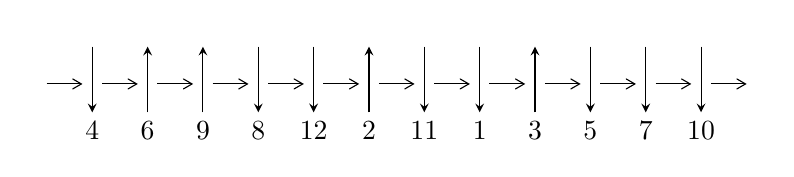
\begin{tikzpicture}[x=20pt, y=17pt]
	% nodes
	\node (C0) at (0, 0) {};
	\node (C1) at (1, 0) {};
	\node (C1U) at (1, +1) {};
	\node (C1D) at (1, -1) {4};

	\node (C2) at (2, 0) {};
	\node (C2U) at (2, +1) {};
	\node (C2D) at (2, -1) {6};

	\node (C3) at (3, 0) {};
	\node (C3U) at (3, +1) {};
	\node (C3D) at (3, -1) {9};

	\node (C4) at (4, 0) {};
	\node (C4U) at (4, +1) {};
	\node (C4D) at (4, -1) {8};

	\node (C5) at (5, 0) {};
	\node (C5U) at (5, +1) {};
	\node (C5D) at (5, -1) {12};

	\node (C6) at (6, 0) {};
	\node (C6U) at (6, +1) {};
	\node (C6D) at (6, -1) {2};

	\node (C7) at (7, 0) {};
	\node (C7U) at (7, +1) {};
	\node (C7D) at (7, -1) {11};

	\node (C8) at (8, 0) {};
	\node (C8U) at (8, +1) {};
	\node (C8D) at (8, -1) {1};

	\node (C9) at (9, 0) {};
	\node (C9U) at (9, +1) {};
	\node (C9D) at (9, -1) {3};

	\node (C10) at (10, 0) {};
	\node (C10U) at (10, +1) {};
	\node (C10D) at (10, -1) {5};

	\node (C11) at (11, 0) {};
	\node (C11U) at (11, +1) {};
	\node (C11D) at (11, -1) {7};

	\node (C12) at (12, 0) {};
	\node (C12U) at (12, +1) {};
	\node (C12D) at (12, -1) {10};
	\node (C13) at (13, 0) {};

	% arrows
	\draw[->,>={angle 60}]
	(C0) edge (C1) (C1) edge (C2) (C2) edge (C3) (C3) edge (C4) (C4) edge (C5) (C5) edge (C6) (C6) edge (C7) (C7) edge (C8) (C8) edge (C9) (C9) edge (C10) (C10) edge (C11) (C11) edge (C12) (C12) edge (C13) ;	\draw[->,>=stealth]
	(C1U) edge (C1D) (C2D) edge (C2U) (C3D) edge (C3U) (C4U) edge (C4D) (C5U) edge (C5D) (C6D) edge (C6U) (C7U) edge (C7D) (C8U) edge (C8D) (C9D) edge (C9U) (C10U) edge (C10D) (C11U) edge (C11D) (C12U) edge (C12D) ;
	\end{tikzpicture} \\
\hhline{~~} \\& 
\textbf{Solving Sequence} \\ \cline{2-2} 
 &
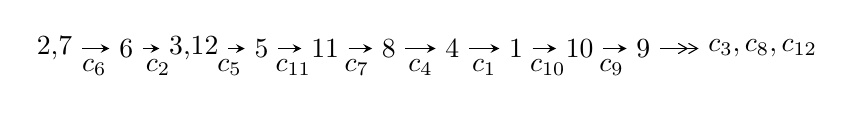
\begin{tikzpicture}[x=23pt, y=7pt]
	% node
	\node (A0) at (-1/8, 0) {2,7};
	\node (A1) at (1, 0) {6};
	\node (A2) at (33/16, 0) {3,12};
	\node (A3) at (25/8, 0) {5};
	\node (A4) at (33/8, 0) {11};
	\node (A5) at (41/8, 0) {8};
	\node (A6) at (49/8, 0) {4};
	\node (A7) at (57/8, 0) {1};
	\node (A8) at (65/8, 0) {10};
	\node (A9) at (73/8, 0) {9};
	\node (C1) at (1/2, -1) {$c_{6}$};
	\node (C2) at (3/2, -1) {$c_{2}$};
	\node (C3) at (21/8, -1) {$c_{5}$};
	\node (C4) at (29/8, -1) {$c_{11}$};
	\node (C5) at (37/8, -1) {$c_{7}$};
	\node (C6) at (45/8, -1) {$c_{4}$};
	\node (C7) at (53/8, -1) {$c_{1}$};
	\node (C8) at (61/8, -1) {$c_{10}$};
	\node (C9) at (69/8, -1) {$c_{9}$};
	\node (A10) at (11, 0) {$c_{3},c_{8},c_{12}$};

	% edge
	\draw[->,>=stealth]	
	(A0) edge (A1) (A1) edge (A2) (A2) edge (A3) (A3) edge (A4) (A4) edge (A5) (A5) edge (A6) (A6) edge (A7) (A7) edge (A8) (A8) edge (A9) ;
	\draw[->>,>={angle 60}]	
	(A9) edge (A10);
\end{tikzpicture} \\ 

\end{tabular} \\

\footnotetext{
The image of knot diagram is generated by the software ``\textbf{Draw programme}" developed by Andrew Bartholomew(\url{http://www.layer8.co.uk/maths/draw/index.htm\#Running-draw}), where we modified some parts for our purpose(\url{https://github.com/CATsTAILs/LinksPainter}).
}\phantom \\ \newline 
\centering \textbf{Ideals for irreducible components\footnotemark of $X_{\text{par}}$} 
 
\begin{align*}
I^u_{1}&=\langle 
-1.26463\times10^{1251} u^{188}-2.01135\times10^{1251} u^{187}+\cdots+1.15374\times10^{1253} b-4.34866\times10^{1255},\\
\phantom{I^u_{1}}&\phantom{= \langle  }-3.65706\times10^{1255} u^{188}-9.37314\times10^{1255} u^{187}+\cdots+6.73843\times10^{1257} a+2.72729\times10^{1260},\\
\phantom{I^u_{1}}&\phantom{= \langle  }u^{189}+2 u^{188}+\cdots+118941 u-58405\rangle \\
I^u_{2}&=\langle 
-9.00364\times10^{53} u^{53}-7.38793\times10^{53} u^{52}+\cdots+4.94949\times10^{51} b+7.82607\times10^{53},\\
\phantom{I^u_{2}}&\phantom{= \langle  }8.75690\times10^{53} u^{53}+3.66837\times10^{53} u^{52}+\cdots+4.94949\times10^{51} a-2.10818\times10^{54},\;u^{54}+u^{53}+\cdots-3 u+1\rangle \\
\\
\end{align*}
\raggedright * 2 irreducible components of $\dim_{\mathbb{C}}=0$, with total 243 representations.\\
\footnotetext{All coefficients of polynomials are rational numbers. But the coefficients are sometimes approximated in decimal forms when there is not enough margin.}
\newpage
\renewcommand{\arraystretch}{1}
\centering \section*{I. $I^u_{1}= \langle -1.26\times10^{1251} u^{188}-2.01\times10^{1251} u^{187}+\cdots+1.15\times10^{1253} b-4.35\times10^{1255},\;-3.66\times10^{1255} u^{188}-9.37\times10^{1255} u^{187}+\cdots+6.74\times10^{1257} a+2.73\times10^{1260},\;u^{189}+2 u^{188}+\cdots+118941 u-58405 \rangle$}
\flushleft \textbf{(i) Arc colorings}\\
\begin{tabular}{m{7pt} m{180pt} m{7pt} m{180pt} }
\flushright $a_{2}=$&$\begin{pmatrix}0\\u\end{pmatrix}$ \\
\flushright $a_{7}=$&$\begin{pmatrix}1\\0\end{pmatrix}$ \\
\flushright $a_{6}=$&$\begin{pmatrix}1\\u^2\end{pmatrix}$ \\
\flushright $a_{3}=$&$\begin{pmatrix}u\\u^3+u\end{pmatrix}$ \\
\flushright $a_{12}=$&$\begin{pmatrix}0.00542717 u^{188}+0.0139100 u^{187}+\cdots+382.471 u-404.738\\0.0109611 u^{188}+0.0174333 u^{187}+\cdots-2251.87 u+376.919\end{pmatrix}$ \\
\flushright $a_{5}=$&$\begin{pmatrix}0.0147816 u^{188}+0.0316648 u^{187}+\cdots-1194.89 u-352.915\\0.00405229 u^{188}+0.00688912 u^{187}+\cdots-711.369 u+48.7705\end{pmatrix}$ \\
\flushright $a_{11}=$&$\begin{pmatrix}0.0163883 u^{188}+0.0313432 u^{187}+\cdots-1869.40 u-27.8189\\0.0109611 u^{188}+0.0174333 u^{187}+\cdots-2251.87 u+376.919\end{pmatrix}$ \\
\flushright $a_{8}=$&$\begin{pmatrix}-0.0112796 u^{188}-0.0197827 u^{187}+\cdots+1435.28 u+26.7246\\-0.00110456 u^{188}-0.00287936 u^{187}+\cdots-292.853 u+152.533\end{pmatrix}$ \\
\flushright $a_{4}=$&$\begin{pmatrix}0.00964069 u^{188}+0.0148069 u^{187}+\cdots-2323.57 u+405.075\\0.00751632 u^{188}+0.0172737 u^{187}+\cdots+12.1275 u-389.388\end{pmatrix}$ \\
\flushright $a_{1}=$&$\begin{pmatrix}-0.0289478 u^{188}-0.0463809 u^{187}+\cdots+5767.71 u-765.938\\-0.0262397 u^{188}-0.0501126 u^{187}+\cdots+2937.81 u+175.792\end{pmatrix}$ \\
\flushright $a_{10}=$&$\begin{pmatrix}-0.00176167 u^{188}+0.0109615 u^{187}+\cdots+4439.35 u-1765.87\\0.00268700 u^{188}+0.0197346 u^{187}+\cdots+4070.65 u-1897.80\end{pmatrix}$ \\
\flushright $a_{9}=$&$\begin{pmatrix}0.00169698 u^{188}+0.0196334 u^{187}+\cdots+4731.83 u-2099.87\\0.00460298 u^{188}+0.0247604 u^{187}+\cdots+4356.43 u-2129.32\end{pmatrix}$\\&\end{tabular}
\flushleft \textbf{(ii) Obstruction class $= -1$}\\~\\
\flushleft \textbf{(iii) Cusp Shapes $= 0.0158544 u^{188}+0.0408087 u^{187}+\cdots-931.471 u-383.977$}\\~\\
\newpage\renewcommand{\arraystretch}{1}
\flushleft \textbf{(iv) u-Polynomials at the component}\newline \\
\begin{tabular}{m{50pt}|m{274pt}}
Crossings & \hspace{64pt}u-Polynomials at each crossing \\
\hline $$\begin{aligned}c_{1}\end{aligned}$$&$\begin{aligned}
&u^{189}-3 u^{188}+\cdots+477364 u-16517
\end{aligned}$\\
\hline $$\begin{aligned}c_{2},c_{6}\end{aligned}$$&$\begin{aligned}
&u^{189}-2 u^{188}+\cdots+118941 u+58405
\end{aligned}$\\
\hline $$\begin{aligned}c_{3},c_{9}\end{aligned}$$&$\begin{aligned}
&u^{189}+u^{188}+\cdots+1777914 u+1267391
\end{aligned}$\\
\hline $$\begin{aligned}c_{4}\end{aligned}$$&$\begin{aligned}
&u^{189}+4 u^{188}+\cdots-64079539000 u+4971467125
\end{aligned}$\\
\hline $$\begin{aligned}c_{5}\end{aligned}$$&$\begin{aligned}
&u^{189}+u^{188}+\cdots+6444964 u+558157
\end{aligned}$\\
\hline $$\begin{aligned}c_{7},c_{11}\end{aligned}$$&$\begin{aligned}
&u^{189}+5 u^{188}+\cdots-572070 u+16507
\end{aligned}$\\
\hline $$\begin{aligned}c_{8}\end{aligned}$$&$\begin{aligned}
&u^{189}+3 u^{188}+\cdots-14 u+1
\end{aligned}$\\
\hline $$\begin{aligned}c_{10}\end{aligned}$$&$\begin{aligned}
&u^{189}+u^{188}+\cdots+50897940 u+7370057
\end{aligned}$\\
\hline $$\begin{aligned}c_{12}\end{aligned}$$&$\begin{aligned}
&u^{189}-15 u^{188}+\cdots-30374880 u+1807073
\end{aligned}$\\
\hline
\end{tabular}\\~\\
\newpage\renewcommand{\arraystretch}{1}
\flushleft \textbf{(v) Riley Polynomials at the component}\newline \\
\begin{tabular}{m{50pt}|m{274pt}}
Crossings & \hspace{64pt}Riley Polynomials at each crossing \\
\hline $$\begin{aligned}c_{1}\end{aligned}$$&$\begin{aligned}
&y^{189}+y^{188}+\cdots+49971649360 y-272811289
\end{aligned}$\\
\hline $$\begin{aligned}c_{2},c_{6}\end{aligned}$$&$\begin{aligned}
&y^{189}+94 y^{188}+\cdots-130612517649 y-3411144025
\end{aligned}$\\
\hline $$\begin{aligned}c_{3},c_{9}\end{aligned}$$&$\begin{aligned}
&y^{189}+135 y^{188}+\cdots-81751009774592 y-1606279946881
\end{aligned}$\\
\hline $$\begin{aligned}c_{4}\end{aligned}$$&$\begin{aligned}
&y^{189}+104 y^{188}+\cdots-1.76\times10^{21} y-2.47\times10^{19}
\end{aligned}$\\
\hline $$\begin{aligned}c_{5}\end{aligned}$$&$\begin{aligned}
&y^{189}+25 y^{188}+\cdots-24262094234224 y-311539236649
\end{aligned}$\\
\hline $$\begin{aligned}c_{7},c_{11}\end{aligned}$$&$\begin{aligned}
&y^{189}+127 y^{188}+\cdots+48428270082 y-272481049
\end{aligned}$\\
\hline $$\begin{aligned}c_{8}\end{aligned}$$&$\begin{aligned}
&y^{189}-5 y^{188}+\cdots+44 y-1
\end{aligned}$\\
\hline $$\begin{aligned}c_{10}\end{aligned}$$&$\begin{aligned}
&y^{189}+53 y^{188}+\cdots-329523948949056 y-54317740183249
\end{aligned}$\\
\hline $$\begin{aligned}c_{12}\end{aligned}$$&$\begin{aligned}
&y^{189}+5 y^{188}+\cdots-213376445564522 y-3265512827329
\end{aligned}$\\
\hline
\end{tabular}\\~\\
\newpage\flushleft \textbf{(vi) Complex Volumes and Cusp Shapes}
$$\begin{array}{c|c|c}  
\text{Solutions to }I^u_{1}& \I (\text{vol} + \sqrt{-1}CS) & \text{Cusp shape}\\
 \hline 
\begin{aligned}
u &= \phantom{-}0.067562 + 0.993666 I \\
a &= -0.267499 - 1.270710 I \\
b &= \phantom{-}0.440694 + 0.994216 I\end{aligned}
 & -0.74624 - 2.81261 I & \phantom{-0.000000 } 0 \\ \hline\begin{aligned}
u &= \phantom{-}0.067562 - 0.993666 I \\
a &= -0.267499 + 1.270710 I \\
b &= \phantom{-}0.440694 - 0.994216 I\end{aligned}
 & -0.74624 + 2.81261 I & \phantom{-0.000000 } 0 \\ \hline\begin{aligned}
u &= \phantom{-}0.630369 + 0.768096 I \\
a &= -2.47900 - 0.30501 I \\
b &= \phantom{-}0.58918 - 1.30282 I\end{aligned}
 & \phantom{-}4.14360 + 8.55032 I & \phantom{-0.000000 } 0 \\ \hline\begin{aligned}
u &= \phantom{-}0.630369 - 0.768096 I \\
a &= -2.47900 + 0.30501 I \\
b &= \phantom{-}0.58918 + 1.30282 I\end{aligned}
 & \phantom{-}4.14360 - 8.55032 I & \phantom{-0.000000 } 0 \\ \hline\begin{aligned}
u &= \phantom{-}0.510576 + 0.847575 I \\
a &= \phantom{-}2.13261 - 0.16877 I \\
b &= -0.63701 + 1.33023 I\end{aligned}
 & \phantom{-}6.20832 + 1.81257 I & \phantom{-0.000000 } 0 \\ \hline\begin{aligned}
u &= \phantom{-}0.510576 - 0.847575 I \\
a &= \phantom{-}2.13261 + 0.16877 I \\
b &= -0.63701 - 1.33023 I\end{aligned}
 & \phantom{-}6.20832 - 1.81257 I & \phantom{-0.000000 } 0 \\ \hline\begin{aligned}
u &= -0.917893 + 0.362064 I \\
a &= \phantom{-}0.127270 + 0.463090 I \\
b &= \phantom{-}0.225853 + 1.222980 I\end{aligned}
 & \phantom{-}3.79380 - 3.29707 I & \phantom{-0.000000 } 0 \\ \hline\begin{aligned}
u &= -0.917893 - 0.362064 I \\
a &= \phantom{-}0.127270 - 0.463090 I \\
b &= \phantom{-}0.225853 - 1.222980 I\end{aligned}
 & \phantom{-}3.79380 + 3.29707 I & \phantom{-0.000000 } 0 \\ \hline\begin{aligned}
u &= -0.194764 + 0.999558 I \\
a &= -1.71200 + 0.32202 I \\
b &= \phantom{-}1.380270 - 0.290565 I\end{aligned}
 & -4.32558 - 0.68091 I & \phantom{-0.000000 } 0 \\ \hline\begin{aligned}
u &= -0.194764 - 0.999558 I \\
a &= -1.71200 - 0.32202 I \\
b &= \phantom{-}1.380270 + 0.290565 I\end{aligned}
 & -4.32558 + 0.68091 I & \phantom{-0.000000 } 0\\
 \hline 
 \end{array}$$\newpage$$\begin{array}{c|c|c}  
\text{Solutions to }I^u_{1}& \I (\text{vol} + \sqrt{-1}CS) & \text{Cusp shape}\\
 \hline 
\begin{aligned}
u &= \phantom{-}0.692832 + 0.691609 I \\
a &= \phantom{-}0.198448 + 0.083327 I \\
b &= \phantom{-}0.41938 + 1.43772 I\end{aligned}
 & \phantom{-}4.30322 - 3.29973 I & \phantom{-0.000000 } 0 \\ \hline\begin{aligned}
u &= \phantom{-}0.692832 - 0.691609 I \\
a &= \phantom{-}0.198448 - 0.083327 I \\
b &= \phantom{-}0.41938 - 1.43772 I\end{aligned}
 & \phantom{-}4.30322 + 3.29973 I & \phantom{-0.000000 } 0 \\ \hline\begin{aligned}
u &= -0.361489 + 0.965972 I \\
a &= \phantom{-}0.732225 - 0.194832 I \\
b &= -0.367068 + 1.340850 I\end{aligned}
 & \phantom{-}3.03261 + 0.04426 I & \phantom{-0.000000 } 0 \\ \hline\begin{aligned}
u &= -0.361489 - 0.965972 I \\
a &= \phantom{-}0.732225 + 0.194832 I \\
b &= -0.367068 - 1.340850 I\end{aligned}
 & \phantom{-}3.03261 - 0.04426 I & \phantom{-0.000000 } 0 \\ \hline\begin{aligned}
u &= \phantom{-}0.454181 + 0.850872 I \\
a &= -1.42130 - 0.79734 I \\
b &= \phantom{-}0.854381 - 0.545454 I\end{aligned}
 & -2.30675 + 2.00402 I & \phantom{-0.000000 } 0 \\ \hline\begin{aligned}
u &= \phantom{-}0.454181 - 0.850872 I \\
a &= -1.42130 + 0.79734 I \\
b &= \phantom{-}0.854381 + 0.545454 I\end{aligned}
 & -2.30675 - 2.00402 I & \phantom{-0.000000 } 0 \\ \hline\begin{aligned}
u &= -0.311636 + 0.911864 I \\
a &= \phantom{-}2.05776 - 1.43772 I \\
b &= -2.05400 + 0.20120 I\end{aligned}
 & -6.91874 - 1.30838 I & \phantom{-0.000000 } 0 \\ \hline\begin{aligned}
u &= -0.311636 - 0.911864 I \\
a &= \phantom{-}2.05776 + 1.43772 I \\
b &= -2.05400 - 0.20120 I\end{aligned}
 & -6.91874 + 1.30838 I & \phantom{-0.000000 } 0 \\ \hline\begin{aligned}
u &= -0.463140 + 0.928696 I \\
a &= \phantom{-}1.16557 - 1.81104 I \\
b &= -0.148287 - 1.207340 I\end{aligned}
 & \phantom{-}3.41518 - 5.11949 I & \phantom{-0.000000 } 0 \\ \hline\begin{aligned}
u &= -0.463140 - 0.928696 I \\
a &= \phantom{-}1.16557 + 1.81104 I \\
b &= -0.148287 + 1.207340 I\end{aligned}
 & \phantom{-}3.41518 + 5.11949 I & \phantom{-0.000000 } 0\\
 \hline 
 \end{array}$$\newpage$$\begin{array}{c|c|c}  
\text{Solutions to }I^u_{1}& \I (\text{vol} + \sqrt{-1}CS) & \text{Cusp shape}\\
 \hline 
\begin{aligned}
u &= -0.800168 + 0.678778 I \\
a &= \phantom{-}0.317561 - 0.373237 I \\
b &= -0.813611 + 0.096392 I\end{aligned}
 & -2.63610 - 2.21131 I & \phantom{-0.000000 } 0 \\ \hline\begin{aligned}
u &= -0.800168 - 0.678778 I \\
a &= \phantom{-}0.317561 + 0.373237 I \\
b &= -0.813611 - 0.096392 I\end{aligned}
 & -2.63610 + 2.21131 I & \phantom{-0.000000 } 0 \\ \hline\begin{aligned}
u &= -0.441877 + 0.835711 I \\
a &= \phantom{-}0.839311 - 0.187778 I \\
b &= -0.072651 + 0.141814 I\end{aligned}
 & -0.04337 - 1.92145 I & \phantom{-0.000000 } 0 \\ \hline\begin{aligned}
u &= -0.441877 - 0.835711 I \\
a &= \phantom{-}0.839311 + 0.187778 I \\
b &= -0.072651 - 0.141814 I\end{aligned}
 & -0.04337 + 1.92145 I & \phantom{-0.000000 } 0 \\ \hline\begin{aligned}
u &= -0.222220 + 1.031650 I \\
a &= \phantom{-}1.60894 - 0.03527 I \\
b &= -0.676095 + 0.053290 I\end{aligned}
 & -1.10304 - 3.13220 I & \phantom{-0.000000 } 0 \\ \hline\begin{aligned}
u &= -0.222220 - 1.031650 I \\
a &= \phantom{-}1.60894 + 0.03527 I \\
b &= -0.676095 - 0.053290 I\end{aligned}
 & -1.10304 + 3.13220 I & \phantom{-0.000000 } 0 \\ \hline\begin{aligned}
u &= -0.178838 + 0.912880 I \\
a &= -1.84808 + 0.39642 I \\
b &= \phantom{-}0.906213 - 0.488177 I\end{aligned}
 & -2.49055 + 0.12903 I & \phantom{-0.000000 } 0 \\ \hline\begin{aligned}
u &= -0.178838 - 0.912880 I \\
a &= -1.84808 - 0.39642 I \\
b &= \phantom{-}0.906213 + 0.488177 I\end{aligned}
 & -2.49055 - 0.12903 I & \phantom{-0.000000 } 0 \\ \hline\begin{aligned}
u &= -1.064960 + 0.179466 I \\
a &= -0.172184 + 0.646048 I \\
b &= \phantom{-}0.951057 + 0.062605 I\end{aligned}
 & -0.33183 + 8.88694 I & \phantom{-0.000000 } 0 \\ \hline\begin{aligned}
u &= -1.064960 - 0.179466 I \\
a &= -0.172184 - 0.646048 I \\
b &= \phantom{-}0.951057 - 0.062605 I\end{aligned}
 & -0.33183 - 8.88694 I & \phantom{-0.000000 } 0\\
 \hline 
 \end{array}$$\newpage$$\begin{array}{c|c|c}  
\text{Solutions to }I^u_{1}& \I (\text{vol} + \sqrt{-1}CS) & \text{Cusp shape}\\
 \hline 
\begin{aligned}
u &= \phantom{-}0.512391 + 0.963034 I \\
a &= -1.53301 - 0.70205 I \\
b &= \phantom{-}0.603849 - 0.418419 I\end{aligned}
 & -3.18405 + 6.17630 I & \phantom{-0.000000 } 0 \\ \hline\begin{aligned}
u &= \phantom{-}0.512391 - 0.963034 I \\
a &= -1.53301 + 0.70205 I \\
b &= \phantom{-}0.603849 + 0.418419 I\end{aligned}
 & -3.18405 - 6.17630 I & \phantom{-0.000000 } 0 \\ \hline\begin{aligned}
u &= \phantom{-}0.519235 + 0.739624 I \\
a &= -0.314813 + 0.480447 I \\
b &= -0.36278 - 1.52314 I\end{aligned}
 & \phantom{-}6.52346 + 2.40126 I & \phantom{-0.000000 } 0 \\ \hline\begin{aligned}
u &= \phantom{-}0.519235 - 0.739624 I \\
a &= -0.314813 - 0.480447 I \\
b &= -0.36278 + 1.52314 I\end{aligned}
 & \phantom{-}6.52346 - 2.40126 I & \phantom{-0.000000 } 0 \\ \hline\begin{aligned}
u &= -0.241346 + 1.071480 I \\
a &= -0.995958 - 0.025369 I \\
b &= \phantom{-}0.919466 - 0.198745 I\end{aligned}
 & -3.20960 - 1.61993 I & \phantom{-0.000000 } 0 \\ \hline\begin{aligned}
u &= -0.241346 - 1.071480 I \\
a &= -0.995958 + 0.025369 I \\
b &= \phantom{-}0.919466 + 0.198745 I\end{aligned}
 & -3.20960 + 1.61993 I & \phantom{-0.000000 } 0 \\ \hline\begin{aligned}
u &= \phantom{-}0.274752 + 1.069880 I \\
a &= -1.29342 - 0.85396 I \\
b &= \phantom{-}1.184690 + 0.383992 I\end{aligned}
 & -5.28303 + 0.39347 I & \phantom{-0.000000 } 0 \\ \hline\begin{aligned}
u &= \phantom{-}0.274752 - 1.069880 I \\
a &= -1.29342 + 0.85396 I \\
b &= \phantom{-}1.184690 - 0.383992 I\end{aligned}
 & -5.28303 - 0.39347 I & \phantom{-0.000000 } 0 \\ \hline\begin{aligned}
u &= \phantom{-}0.000937 + 1.113790 I \\
a &= \phantom{-}0.551845 + 0.591997 I \\
b &= -0.12195 + 1.44938 I\end{aligned}
 & \phantom{-}3.37739 + 0.05370 I & \phantom{-0.000000 } 0 \\ \hline\begin{aligned}
u &= \phantom{-}0.000937 - 1.113790 I \\
a &= \phantom{-}0.551845 - 0.591997 I \\
b &= -0.12195 - 1.44938 I\end{aligned}
 & \phantom{-}3.37739 - 0.05370 I & \phantom{-0.000000 } 0\\
 \hline 
 \end{array}$$\newpage$$\begin{array}{c|c|c}  
\text{Solutions to }I^u_{1}& \I (\text{vol} + \sqrt{-1}CS) & \text{Cusp shape}\\
 \hline 
\begin{aligned}
u &= \phantom{-}1.044860 + 0.385777 I \\
a &= \phantom{-}0.080676 - 0.219129 I \\
b &= -0.433531 - 1.319580 I\end{aligned}
 & \phantom{-}7.58545 - 8.67350 I & \phantom{-0.000000 } 0 \\ \hline\begin{aligned}
u &= \phantom{-}1.044860 - 0.385777 I \\
a &= \phantom{-}0.080676 + 0.219129 I \\
b &= -0.433531 + 1.319580 I\end{aligned}
 & \phantom{-}7.58545 + 8.67350 I & \phantom{-0.000000 } 0 \\ \hline\begin{aligned}
u &= \phantom{-}0.880213 + 0.084755 I \\
a &= \phantom{-}0.661929 + 0.103970 I \\
b &= -0.218737 - 1.077910 I\end{aligned}
 & -0.40974 - 6.70785 I & \phantom{-0.000000 } 0 \\ \hline\begin{aligned}
u &= \phantom{-}0.880213 - 0.084755 I \\
a &= \phantom{-}0.661929 - 0.103970 I \\
b &= -0.218737 + 1.077910 I\end{aligned}
 & -0.40974 + 6.70785 I & \phantom{-0.000000 } 0 \\ \hline\begin{aligned}
u &= \phantom{-}0.344219 + 0.809766 I \\
a &= \phantom{-}0.630549 + 0.772802 I \\
b &= -0.247227 + 0.493087 I\end{aligned}
 & -0.30431 - 2.06669 I & \phantom{-0.000000 } 0 \\ \hline\begin{aligned}
u &= \phantom{-}0.344219 - 0.809766 I \\
a &= \phantom{-}0.630549 - 0.772802 I \\
b &= -0.247227 - 0.493087 I\end{aligned}
 & -0.30431 + 2.06669 I & \phantom{-0.000000 } 0 \\ \hline\begin{aligned}
u &= -1.118940 + 0.108725 I \\
a &= \phantom{-}0.183365 - 0.289602 I \\
b &= -0.178442 - 1.248700 I\end{aligned}
 & \phantom{-}7.17662 - 2.58172 I & \phantom{-0.000000 } 0 \\ \hline\begin{aligned}
u &= -1.118940 - 0.108725 I \\
a &= \phantom{-}0.183365 + 0.289602 I \\
b &= -0.178442 + 1.248700 I\end{aligned}
 & \phantom{-}7.17662 + 2.58172 I & \phantom{-0.000000 } 0 \\ \hline\begin{aligned}
u &= \phantom{-}0.233385 + 1.102620 I \\
a &= -1.070960 - 0.124060 I \\
b &= \phantom{-}0.144351 + 0.461703 I\end{aligned}
 & -1.09068 + 3.64692 I & \phantom{-0.000000 } 0 \\ \hline\begin{aligned}
u &= \phantom{-}0.233385 - 1.102620 I \\
a &= -1.070960 + 0.124060 I \\
b &= \phantom{-}0.144351 - 0.461703 I\end{aligned}
 & -1.09068 - 3.64692 I & \phantom{-0.000000 } 0\\
 \hline 
 \end{array}$$\newpage$$\begin{array}{c|c|c}  
\text{Solutions to }I^u_{1}& \I (\text{vol} + \sqrt{-1}CS) & \text{Cusp shape}\\
 \hline 
\begin{aligned}
u &= -0.446277 + 1.038550 I \\
a &= \phantom{-}0.050035 + 0.499135 I \\
b &= \phantom{-}0.48444 - 1.70775 I\end{aligned}
 & \phantom{-}1.80645 - 7.56881 I & \phantom{-0.000000 } 0 \\ \hline\begin{aligned}
u &= -0.446277 - 1.038550 I \\
a &= \phantom{-}0.050035 - 0.499135 I \\
b &= \phantom{-}0.48444 + 1.70775 I\end{aligned}
 & \phantom{-}1.80645 + 7.56881 I & \phantom{-0.000000 } 0 \\ \hline\begin{aligned}
u &= \phantom{-}1.115130 + 0.245711 I \\
a &= -0.182423 - 0.710528 I \\
b &= \phantom{-}0.809625 - 0.110733 I\end{aligned}
 & \phantom{-}0.60913 + 3.47500 I & \phantom{-0.000000 } 0 \\ \hline\begin{aligned}
u &= \phantom{-}1.115130 - 0.245711 I \\
a &= -0.182423 + 0.710528 I \\
b &= \phantom{-}0.809625 + 0.110733 I\end{aligned}
 & \phantom{-}0.60913 - 3.47500 I & \phantom{-0.000000 } 0 \\ \hline\begin{aligned}
u &= -0.592722 + 0.978809 I \\
a &= -0.127519 + 0.773384 I \\
b &= -0.12252 + 1.43050 I\end{aligned}
 & \phantom{-}2.61438 + 1.30056 I & \phantom{-0.000000 } 0 \\ \hline\begin{aligned}
u &= -0.592722 - 0.978809 I \\
a &= -0.127519 - 0.773384 I \\
b &= -0.12252 - 1.43050 I\end{aligned}
 & \phantom{-}2.61438 - 1.30056 I & \phantom{-0.000000 } 0 \\ \hline\begin{aligned}
u &= \phantom{-}0.390097 + 1.081100 I \\
a &= -0.64874 - 1.46046 I \\
b &= \phantom{-}0.119477 - 1.312790 I\end{aligned}
 & \phantom{-}0.92326 + 9.92067 I & \phantom{-0.000000 } 0 \\ \hline\begin{aligned}
u &= \phantom{-}0.390097 - 1.081100 I \\
a &= -0.64874 + 1.46046 I \\
b &= \phantom{-}0.119477 + 1.312790 I\end{aligned}
 & \phantom{-}0.92326 - 9.92067 I & \phantom{-0.000000 } 0 \\ \hline\begin{aligned}
u &= -0.471385 + 0.705543 I \\
a &= \phantom{-}3.38266 - 0.86554 I \\
b &= \phantom{-}0.007629 - 1.191340 I\end{aligned}
 & \phantom{-}3.50830 - 5.62560 I & \phantom{-0.000000 } 0 \\ \hline\begin{aligned}
u &= -0.471385 - 0.705543 I \\
a &= \phantom{-}3.38266 + 0.86554 I \\
b &= \phantom{-}0.007629 + 1.191340 I\end{aligned}
 & \phantom{-}3.50830 + 5.62560 I & \phantom{-0.000000 } 0\\
 \hline 
 \end{array}$$\newpage$$\begin{array}{c|c|c}  
\text{Solutions to }I^u_{1}& \I (\text{vol} + \sqrt{-1}CS) & \text{Cusp shape}\\
 \hline 
\begin{aligned}
u &= \phantom{-}0.408891 + 1.077710 I \\
a &= \phantom{-}1.34024 + 0.54291 I \\
b &= -0.754514 - 0.492258 I\end{aligned}
 & -5.42324 + 7.41959 I & \phantom{-0.000000 } 0 \\ \hline\begin{aligned}
u &= \phantom{-}0.408891 - 1.077710 I \\
a &= \phantom{-}1.34024 - 0.54291 I \\
b &= -0.754514 + 0.492258 I\end{aligned}
 & -5.42324 - 7.41959 I & \phantom{-0.000000 } 0 \\ \hline\begin{aligned}
u &= -0.381832 + 0.750348 I \\
a &= -3.21827 + 1.18751 I \\
b &= -0.040379 + 1.009940 I\end{aligned}
 & \phantom{-}4.06792 + 1.50761 I & \phantom{-0.000000 } 0 \\ \hline\begin{aligned}
u &= -0.381832 - 0.750348 I \\
a &= -3.21827 - 1.18751 I \\
b &= -0.040379 - 1.009940 I\end{aligned}
 & \phantom{-}4.06792 - 1.50761 I & \phantom{-0.000000 } 0 \\ \hline\begin{aligned}
u &= -0.354456 + 0.760501 I \\
a &= \phantom{-}0.696321 + 0.178152 I \\
b &= -0.085884 + 0.266995 I\end{aligned}
 & \phantom{-}0.15883 - 1.69167 I & \phantom{-0.000000 } 0 \\ \hline\begin{aligned}
u &= -0.354456 - 0.760501 I \\
a &= \phantom{-}0.696321 - 0.178152 I \\
b &= -0.085884 - 0.266995 I\end{aligned}
 & \phantom{-}0.15883 + 1.69167 I & \phantom{-0.000000 } 0 \\ \hline\begin{aligned}
u &= \phantom{-}0.765705 + 0.882418 I \\
a &= -1.074670 - 0.891398 I \\
b &= \phantom{-}0.247833 - 0.841024 I\end{aligned}
 & -2.95144 + 6.03869 I & \phantom{-0.000000 } 0 \\ \hline\begin{aligned}
u &= \phantom{-}0.765705 - 0.882418 I \\
a &= -1.074670 + 0.891398 I \\
b &= \phantom{-}0.247833 + 0.841024 I\end{aligned}
 & -2.95144 - 6.03869 I & \phantom{-0.000000 } 0 \\ \hline\begin{aligned}
u &= \phantom{-}0.617135 + 1.003760 I \\
a &= -1.069770 - 0.816316 I \\
b &= \phantom{-}1.306430 + 0.027422 I\end{aligned}
 & -1.15137 + 2.76544 I & \phantom{-0.000000 } 0 \\ \hline\begin{aligned}
u &= \phantom{-}0.617135 - 1.003760 I \\
a &= -1.069770 + 0.816316 I \\
b &= \phantom{-}1.306430 - 0.027422 I\end{aligned}
 & -1.15137 - 2.76544 I & \phantom{-0.000000 } 0\\
 \hline 
 \end{array}$$\newpage$$\begin{array}{c|c|c}  
\text{Solutions to }I^u_{1}& \I (\text{vol} + \sqrt{-1}CS) & \text{Cusp shape}\\
 \hline 
\begin{aligned}
u &= -0.522093 + 1.061040 I \\
a &= \phantom{-}1.314740 + 0.346065 I \\
b &= -0.241299 - 0.745231 I\end{aligned}
 & \phantom{-}0.46504 - 2.65571 I & \phantom{-0.000000 } 0 \\ \hline\begin{aligned}
u &= -0.522093 - 1.061040 I \\
a &= \phantom{-}1.314740 - 0.346065 I \\
b &= -0.241299 + 0.745231 I\end{aligned}
 & \phantom{-}0.46504 + 2.65571 I & \phantom{-0.000000 } 0 \\ \hline\begin{aligned}
u &= -0.383872 + 1.124090 I \\
a &= -1.65439 - 0.84100 I \\
b &= \phantom{-}0.477323 + 0.993956 I\end{aligned}
 & -0.87929 - 4.94706 I & \phantom{-0.000000 } 0 \\ \hline\begin{aligned}
u &= -0.383872 - 1.124090 I \\
a &= -1.65439 + 0.84100 I \\
b &= \phantom{-}0.477323 - 0.993956 I\end{aligned}
 & -0.87929 + 4.94706 I & \phantom{-0.000000 } 0 \\ \hline\begin{aligned}
u &= -0.580358 + 1.043430 I \\
a &= \phantom{-}1.94397 - 0.08820 I \\
b &= -0.118806 - 1.152000 I\end{aligned}
 & \phantom{-}2.68465 - 3.07609 I & \phantom{-0.000000 } 0 \\ \hline\begin{aligned}
u &= -0.580358 - 1.043430 I \\
a &= \phantom{-}1.94397 + 0.08820 I \\
b &= -0.118806 + 1.152000 I\end{aligned}
 & \phantom{-}2.68465 + 3.07609 I & \phantom{-0.000000 } 0 \\ \hline\begin{aligned}
u &= \phantom{-}0.156852 + 0.790567 I \\
a &= -3.36753 + 1.61930 I \\
b &= -0.011186 - 1.047930 I\end{aligned}
 & \phantom{-}4.28093 + 1.14181 I & \phantom{-0.000000 } 0 \\ \hline\begin{aligned}
u &= \phantom{-}0.156852 - 0.790567 I \\
a &= -3.36753 - 1.61930 I \\
b &= -0.011186 + 1.047930 I\end{aligned}
 & \phantom{-}4.28093 - 1.14181 I & \phantom{-0.000000 } 0 \\ \hline\begin{aligned}
u &= \phantom{-}0.679730 + 0.427112 I \\
a &= -0.067595 + 0.748744 I \\
b &= \phantom{-}0.28865 + 1.45093 I\end{aligned}
 & \phantom{-}4.58859 - 5.52276 I & \phantom{-0.000000 } 0 \\ \hline\begin{aligned}
u &= \phantom{-}0.679730 - 0.427112 I \\
a &= -0.067595 - 0.748744 I \\
b &= \phantom{-}0.28865 - 1.45093 I\end{aligned}
 & \phantom{-}4.58859 + 5.52276 I & \phantom{-0.000000 } 0\\
 \hline 
 \end{array}$$\newpage$$\begin{array}{c|c|c}  
\text{Solutions to }I^u_{1}& \I (\text{vol} + \sqrt{-1}CS) & \text{Cusp shape}\\
 \hline 
\begin{aligned}
u &= -0.716346 + 0.357965 I \\
a &= \phantom{-}0.660286 + 0.769140 I \\
b &= \phantom{-}0.035944 + 1.226680 I\end{aligned}
 & \phantom{-}4.49713 - 1.77571 I & \phantom{-0.000000 } 0 \\ \hline\begin{aligned}
u &= -0.716346 - 0.357965 I \\
a &= \phantom{-}0.660286 - 0.769140 I \\
b &= \phantom{-}0.035944 - 1.226680 I\end{aligned}
 & \phantom{-}4.49713 + 1.77571 I & \phantom{-0.000000 } 0 \\ \hline\begin{aligned}
u &= -0.493820 + 1.099010 I \\
a &= \phantom{-}1.77862 + 0.09146 I \\
b &= -0.64187 - 1.60029 I\end{aligned}
 & -1.31049 - 10.22440 I & \phantom{-0.000000 } 0 \\ \hline\begin{aligned}
u &= -0.493820 - 1.099010 I \\
a &= \phantom{-}1.77862 - 0.09146 I \\
b &= -0.64187 + 1.60029 I\end{aligned}
 & -1.31049 + 10.22440 I & \phantom{-0.000000 } 0 \\ \hline\begin{aligned}
u &= -0.352654 + 1.152340 I \\
a &= \phantom{-}0.257122 - 0.544690 I \\
b &= -0.725173 + 0.970993 I\end{aligned}
 & -2.05464 + 2.54881 I & \phantom{-0.000000 } 0 \\ \hline\begin{aligned}
u &= -0.352654 - 1.152340 I \\
a &= \phantom{-}0.257122 + 0.544690 I \\
b &= -0.725173 - 0.970993 I\end{aligned}
 & -2.05464 - 2.54881 I & \phantom{-0.000000 } 0 \\ \hline\begin{aligned}
u &= \phantom{-}0.512946 + 1.094040 I \\
a &= \phantom{-}1.30527 + 0.60900 I \\
b &= -1.225240 - 0.084845 I\end{aligned}
 & \phantom{-}0.88755 + 8.48409 I & \phantom{-0.000000 } 0 \\ \hline\begin{aligned}
u &= \phantom{-}0.512946 - 1.094040 I \\
a &= \phantom{-}1.30527 - 0.60900 I \\
b &= -1.225240 + 0.084845 I\end{aligned}
 & \phantom{-}0.88755 - 8.48409 I & \phantom{-0.000000 } 0 \\ \hline\begin{aligned}
u &= \phantom{-}1.217460 + 0.149329 I \\
a &= -0.510262 + 0.513572 I \\
b &= -0.025895 + 1.015500 I\end{aligned}
 & \phantom{-}4.82411 + 0.12862 I & \phantom{-0.000000 } 0 \\ \hline\begin{aligned}
u &= \phantom{-}1.217460 - 0.149329 I \\
a &= -0.510262 - 0.513572 I \\
b &= -0.025895 - 1.015500 I\end{aligned}
 & \phantom{-}4.82411 - 0.12862 I & \phantom{-0.000000 } 0\\
 \hline 
 \end{array}$$\newpage$$\begin{array}{c|c|c}  
\text{Solutions to }I^u_{1}& \I (\text{vol} + \sqrt{-1}CS) & \text{Cusp shape}\\
 \hline 
\begin{aligned}
u &= -0.432266 + 1.148690 I \\
a &= \phantom{-}0.007625 - 0.552867 I \\
b &= -0.0840058 - 0.0007714 I\end{aligned}
 & -0.01218 - 3.75481 I & \phantom{-0.000000 } 0 \\ \hline\begin{aligned}
u &= -0.432266 - 1.148690 I \\
a &= \phantom{-}0.007625 + 0.552867 I \\
b &= -0.0840058 + 0.0007714 I\end{aligned}
 & -0.01218 + 3.75481 I & \phantom{-0.000000 } 0 \\ \hline\begin{aligned}
u &= \phantom{-}0.576994 + 1.088980 I \\
a &= -2.01481 + 0.00072 I \\
b &= \phantom{-}0.40800 - 1.45334 I\end{aligned}
 & \phantom{-}2.63633 + 10.42350 I & \phantom{-0.000000 } 0 \\ \hline\begin{aligned}
u &= \phantom{-}0.576994 - 1.088980 I \\
a &= -2.01481 - 0.00072 I \\
b &= \phantom{-}0.40800 + 1.45334 I\end{aligned}
 & \phantom{-}2.63633 - 10.42350 I & \phantom{-0.000000 } 0 \\ \hline\begin{aligned}
u &= -0.076030 + 1.236970 I \\
a &= \phantom{-}1.396020 - 0.078850 I \\
b &= -0.892554 - 0.514801 I\end{aligned}
 & -8.87914 - 3.86366 I & \phantom{-0.000000 } 0 \\ \hline\begin{aligned}
u &= -0.076030 - 1.236970 I \\
a &= \phantom{-}1.396020 + 0.078850 I \\
b &= -0.892554 + 0.514801 I\end{aligned}
 & -8.87914 + 3.86366 I & \phantom{-0.000000 } 0 \\ \hline\begin{aligned}
u &= \phantom{-}0.258678 + 1.229290 I \\
a &= \phantom{-}0.180358 - 0.797563 I \\
b &= \phantom{-}0.102146 + 1.087260 I\end{aligned}
 & \phantom{-}0.45441 - 2.90483 I & \phantom{-0.000000 } 0 \\ \hline\begin{aligned}
u &= \phantom{-}0.258678 - 1.229290 I \\
a &= \phantom{-}0.180358 + 0.797563 I \\
b &= \phantom{-}0.102146 - 1.087260 I\end{aligned}
 & \phantom{-}0.45441 + 2.90483 I & \phantom{-0.000000 } 0 \\ \hline\begin{aligned}
u &= \phantom{-}0.672787 + 0.309542 I \\
a &= \phantom{-}0.263570 + 0.645799 I \\
b &= \phantom{-}0.317339 + 0.771337 I\end{aligned}
 & -0.61250 - 1.94201 I & \phantom{-0.000000 } 0 \\ \hline\begin{aligned}
u &= \phantom{-}0.672787 - 0.309542 I \\
a &= \phantom{-}0.263570 - 0.645799 I \\
b &= \phantom{-}0.317339 - 0.771337 I\end{aligned}
 & -0.61250 + 1.94201 I & \phantom{-0.000000 } 0\\
 \hline 
 \end{array}$$\newpage$$\begin{array}{c|c|c}  
\text{Solutions to }I^u_{1}& \I (\text{vol} + \sqrt{-1}CS) & \text{Cusp shape}\\
 \hline 
\begin{aligned}
u &= -0.441217 + 1.182520 I \\
a &= \phantom{-}1.71510 + 0.52130 I \\
b &= -0.395486 - 1.312000 I\end{aligned}
 & \phantom{-}2.93433 - 7.19351 I & \phantom{-0.000000 } 0 \\ \hline\begin{aligned}
u &= -0.441217 - 1.182520 I \\
a &= \phantom{-}1.71510 - 0.52130 I \\
b &= -0.395486 + 1.312000 I\end{aligned}
 & \phantom{-}2.93433 + 7.19351 I & \phantom{-0.000000 } 0 \\ \hline\begin{aligned}
u &= -0.722100 + 0.139284 I \\
a &= \phantom{-}0.216267 + 0.787891 I \\
b &= -0.442679 - 0.213941 I\end{aligned}
 & \phantom{-}2.91455 - 0.44704 I & \phantom{-0.000000 } 0 \\ \hline\begin{aligned}
u &= -0.722100 - 0.139284 I \\
a &= \phantom{-}0.216267 - 0.787891 I \\
b &= -0.442679 + 0.213941 I\end{aligned}
 & \phantom{-}2.91455 + 0.44704 I & \phantom{-0.000000 } 0 \\ \hline\begin{aligned}
u &= \phantom{-}0.569076 + 1.130950 I \\
a &= -1.48674 - 0.31305 I \\
b &= \phantom{-}0.648890 - 1.097580 I\end{aligned}
 & -3.00359 + 6.86673 I & \phantom{-0.000000 } 0 \\ \hline\begin{aligned}
u &= \phantom{-}0.569076 - 1.130950 I \\
a &= -1.48674 + 0.31305 I \\
b &= \phantom{-}0.648890 + 1.097580 I\end{aligned}
 & -3.00359 - 6.86673 I & \phantom{-0.000000 } 0 \\ \hline\begin{aligned}
u &= \phantom{-}0.655347 + 0.309483 I \\
a &= \phantom{-}0.413478 + 1.052100 I \\
b &= -0.882636 - 0.151125 I\end{aligned}
 & \phantom{-}3.12881 - 3.97775 I & \phantom{-0.000000 } 0 \\ \hline\begin{aligned}
u &= \phantom{-}0.655347 - 0.309483 I \\
a &= \phantom{-}0.413478 - 1.052100 I \\
b &= -0.882636 + 0.151125 I\end{aligned}
 & \phantom{-}3.12881 + 3.97775 I & \phantom{-0.000000 } 0 \\ \hline\begin{aligned}
u &= -0.693295 + 1.076160 I \\
a &= \phantom{-}1.212590 - 0.146757 I \\
b &= -0.065535 - 1.034750 I\end{aligned}
 & \phantom{-}1.82503 - 2.62563 I & \phantom{-0.000000 } 0 \\ \hline\begin{aligned}
u &= -0.693295 - 1.076160 I \\
a &= \phantom{-}1.212590 + 0.146757 I \\
b &= -0.065535 + 1.034750 I\end{aligned}
 & \phantom{-}1.82503 + 2.62563 I & \phantom{-0.000000 } 0\\
 \hline 
 \end{array}$$\newpage$$\begin{array}{c|c|c}  
\text{Solutions to }I^u_{1}& \I (\text{vol} + \sqrt{-1}CS) & \text{Cusp shape}\\
 \hline 
\begin{aligned}
u &= \phantom{-}0.608820 + 1.129940 I \\
a &= \phantom{-}0.982819 + 0.606534 I \\
b &= -0.194681 + 1.006450 I\end{aligned}
 & -4.10244 - 0.46469 I & \phantom{-0.000000 } 0 \\ \hline\begin{aligned}
u &= \phantom{-}0.608820 - 1.129940 I \\
a &= \phantom{-}0.982819 - 0.606534 I \\
b &= -0.194681 - 1.006450 I\end{aligned}
 & -4.10244 + 0.46469 I & \phantom{-0.000000 } 0 \\ \hline\begin{aligned}
u &= -0.737424 + 1.056050 I \\
a &= \phantom{-}0.969367 - 0.664757 I \\
b &= -1.047580 - 0.520281 I\end{aligned}
 & -3.68053 - 3.71422 I & \phantom{-0.000000 } 0 \\ \hline\begin{aligned}
u &= -0.737424 - 1.056050 I \\
a &= \phantom{-}0.969367 + 0.664757 I \\
b &= -1.047580 + 0.520281 I\end{aligned}
 & -3.68053 + 3.71422 I & \phantom{-0.000000 } 0 \\ \hline\begin{aligned}
u &= -0.091255 + 0.706063 I \\
a &= -1.59937 - 0.41719 I \\
b &= \phantom{-}0.336292 - 1.296860 I\end{aligned}
 & \phantom{-}1.36934 + 2.64236 I & \phantom{-0.000000 } 0 \\ \hline\begin{aligned}
u &= -0.091255 - 0.706063 I \\
a &= -1.59937 + 0.41719 I \\
b &= \phantom{-}0.336292 + 1.296860 I\end{aligned}
 & \phantom{-}1.36934 - 2.64236 I & \phantom{-0.000000 } 0 \\ \hline\begin{aligned}
u &= -0.384288 + 0.593663 I \\
a &= -3.52724 - 0.48755 I \\
b &= \phantom{-}0.62491 + 1.28264 I\end{aligned}
 & \phantom{-}3.31040 + 3.95615 I & \phantom{-0.000000 } 0 \\ \hline\begin{aligned}
u &= -0.384288 - 0.593663 I \\
a &= -3.52724 + 0.48755 I \\
b &= \phantom{-}0.62491 - 1.28264 I\end{aligned}
 & \phantom{-}3.31040 - 3.95615 I & \phantom{-0.000000 } 0 \\ \hline\begin{aligned}
u &= -0.369249 + 0.588410 I \\
a &= \phantom{-}2.95522 + 0.82669 I \\
b &= -0.638871 - 1.005640 I\end{aligned}
 & \phantom{-}4.31988 - 3.35233 I & \phantom{-0.000000 } 0 \\ \hline\begin{aligned}
u &= -0.369249 - 0.588410 I \\
a &= \phantom{-}2.95522 - 0.82669 I \\
b &= -0.638871 + 1.005640 I\end{aligned}
 & \phantom{-}4.31988 + 3.35233 I & \phantom{-0.000000 } 0\\
 \hline 
 \end{array}$$\newpage$$\begin{array}{c|c|c}  
\text{Solutions to }I^u_{1}& \I (\text{vol} + \sqrt{-1}CS) & \text{Cusp shape}\\
 \hline 
\begin{aligned}
u &= -0.643352 + 0.255879 I \\
a &= \phantom{-}0.215868 - 0.127431 I \\
b &= \phantom{-}0.078573 + 1.100240 I\end{aligned}
 & \phantom{-}2.69451 - 1.80792 I & \phantom{-0.000000 } 0 \\ \hline\begin{aligned}
u &= -0.643352 - 0.255879 I \\
a &= \phantom{-}0.215868 + 0.127431 I \\
b &= \phantom{-}0.078573 - 1.100240 I\end{aligned}
 & \phantom{-}2.69451 + 1.80792 I & \phantom{-0.000000 } 0 \\ \hline\begin{aligned}
u &= \phantom{-}0.730727 + 1.084910 I \\
a &= -1.75951 - 0.24757 I \\
b &= \phantom{-}0.54865 - 1.41013 I\end{aligned}
 & \phantom{-}3.42042 + 9.10061 I & \phantom{-0.000000 } 0 \\ \hline\begin{aligned}
u &= \phantom{-}0.730727 - 1.084910 I \\
a &= -1.75951 + 0.24757 I \\
b &= \phantom{-}0.54865 + 1.41013 I\end{aligned}
 & \phantom{-}3.42042 - 9.10061 I & \phantom{-0.000000 } 0 \\ \hline\begin{aligned}
u &= \phantom{-}0.505679 + 1.208570 I \\
a &= -1.76259 + 0.06068 I \\
b &= \phantom{-}0.178992 - 1.132550 I\end{aligned}
 & \phantom{-}1.07343 + 5.25271 I & \phantom{-0.000000 } 0 \\ \hline\begin{aligned}
u &= \phantom{-}0.505679 - 1.208570 I \\
a &= -1.76259 - 0.06068 I \\
b &= \phantom{-}0.178992 + 1.132550 I\end{aligned}
 & \phantom{-}1.07343 - 5.25271 I & \phantom{-0.000000 } 0 \\ \hline\begin{aligned}
u &= -1.284040 + 0.266390 I \\
a &= \phantom{-}0.302786 - 0.263434 I \\
b &= \phantom{-}0.327306 - 1.027510 I\end{aligned}
 & \phantom{-}3.41150 + 1.29969 I & \phantom{-0.000000 } 0 \\ \hline\begin{aligned}
u &= -1.284040 - 0.266390 I \\
a &= \phantom{-}0.302786 + 0.263434 I \\
b &= \phantom{-}0.327306 + 1.027510 I\end{aligned}
 & \phantom{-}3.41150 - 1.29969 I & \phantom{-0.000000 } 0 \\ \hline\begin{aligned}
u &= \phantom{-}0.554587 + 1.191530 I \\
a &= -0.498696 - 0.301605 I \\
b &= \phantom{-}0.671956 + 0.459612 I\end{aligned}
 & -3.89674 + 2.00708 I & \phantom{-0.000000 } 0 \\ \hline\begin{aligned}
u &= \phantom{-}0.554587 - 1.191530 I \\
a &= -0.498696 + 0.301605 I \\
b &= \phantom{-}0.671956 - 0.459612 I\end{aligned}
 & -3.89674 - 2.00708 I & \phantom{-0.000000 } 0\\
 \hline 
 \end{array}$$\newpage$$\begin{array}{c|c|c}  
\text{Solutions to }I^u_{1}& \I (\text{vol} + \sqrt{-1}CS) & \text{Cusp shape}\\
 \hline 
\begin{aligned}
u &= \phantom{-}0.268575 + 0.629923 I \\
a &= \phantom{-}5.08122 - 0.37331 I \\
b &= \phantom{-}0.123893 + 1.026060 I\end{aligned}
 & \phantom{-}2.63860 - 6.93401 I & \phantom{-0.000000 } 0 \\ \hline\begin{aligned}
u &= \phantom{-}0.268575 - 0.629923 I \\
a &= \phantom{-}5.08122 + 0.37331 I \\
b &= \phantom{-}0.123893 - 1.026060 I\end{aligned}
 & \phantom{-}2.63860 + 6.93401 I & \phantom{-0.000000 } 0 \\ \hline\begin{aligned}
u &= -0.463069 + 1.233500 I \\
a &= -1.40411 - 0.42836 I \\
b &= \phantom{-}0.65767 + 1.34438 I\end{aligned}
 & -0.72991 - 7.65659 I & \phantom{-0.000000 } 0 \\ \hline\begin{aligned}
u &= -0.463069 - 1.233500 I \\
a &= -1.40411 + 0.42836 I \\
b &= \phantom{-}0.65767 - 1.34438 I\end{aligned}
 & -0.72991 + 7.65659 I & \phantom{-0.000000 } 0 \\ \hline\begin{aligned}
u &= \phantom{-}0.532497 + 1.209700 I \\
a &= \phantom{-}1.87562 - 0.38555 I \\
b &= -0.398682 + 1.054470 I\end{aligned}
 & -3.67796 + 11.75010 I & \phantom{-0.000000 } 0 \\ \hline\begin{aligned}
u &= \phantom{-}0.532497 - 1.209700 I \\
a &= \phantom{-}1.87562 + 0.38555 I \\
b &= -0.398682 - 1.054470 I\end{aligned}
 & -3.67796 - 11.75010 I & \phantom{-0.000000 } 0 \\ \hline\begin{aligned}
u &= -0.074654 + 0.660263 I \\
a &= -0.248672 + 0.959306 I \\
b &= -0.17057 + 1.47829 I\end{aligned}
 & \phantom{-}5.76126 + 4.77365 I & \phantom{-0.000000 } 0 \\ \hline\begin{aligned}
u &= -0.074654 - 0.660263 I \\
a &= -0.248672 - 0.959306 I \\
b &= -0.17057 - 1.47829 I\end{aligned}
 & \phantom{-}5.76126 - 4.77365 I & \phantom{-0.000000 } 0 \\ \hline\begin{aligned}
u &= -1.259640 + 0.464351 I \\
a &= -0.116615 - 0.297780 I \\
b &= \phantom{-}0.509769 - 1.307060 I\end{aligned}
 & \phantom{-}3.5415 + 14.1773 I & \phantom{-0.000000 } 0 \\ \hline\begin{aligned}
u &= -1.259640 - 0.464351 I \\
a &= -0.116615 + 0.297780 I \\
b &= \phantom{-}0.509769 + 1.307060 I\end{aligned}
 & \phantom{-}3.5415 - 14.1773 I & \phantom{-0.000000 } 0\\
 \hline 
 \end{array}$$\newpage$$\begin{array}{c|c|c}  
\text{Solutions to }I^u_{1}& \I (\text{vol} + \sqrt{-1}CS) & \text{Cusp shape}\\
 \hline 
\begin{aligned}
u &= \phantom{-}0.546779 + 0.319380 I \\
a &= \phantom{-}0.163842 + 0.122860 I \\
b &= \phantom{-}0.682547 + 0.440816 I\end{aligned}
 & -1.53356 - 1.95289 I & \phantom{-0.000000 } 0 \\ \hline\begin{aligned}
u &= \phantom{-}0.546779 - 0.319380 I \\
a &= \phantom{-}0.163842 - 0.122860 I \\
b &= \phantom{-}0.682547 - 0.440816 I\end{aligned}
 & -1.53356 + 1.95289 I & \phantom{-0.000000 } 0 \\ \hline\begin{aligned}
u &= \phantom{-}0.089516 + 0.625740 I \\
a &= -0.383413 + 0.642993 I \\
b &= \phantom{-}0.18268 - 1.61150 I\end{aligned}
 & \phantom{-}3.15914 + 5.21994 I & \phantom{-0.000000 } 0 \\ \hline\begin{aligned}
u &= \phantom{-}0.089516 - 0.625740 I \\
a &= -0.383413 - 0.642993 I \\
b &= \phantom{-}0.18268 + 1.61150 I\end{aligned}
 & \phantom{-}3.15914 - 5.21994 I & \phantom{-0.000000 } 0 \\ \hline\begin{aligned}
u &= -0.543527 + 0.304729 I \\
a &= \phantom{-}0.76298 - 2.01736 I \\
b &= -0.357184 - 1.283810 I\end{aligned}
 & \phantom{-}1.11652 - 6.49918 I & \phantom{-0.000000 } 0 \\ \hline\begin{aligned}
u &= -0.543527 - 0.304729 I \\
a &= \phantom{-}0.76298 + 2.01736 I \\
b &= -0.357184 + 1.283810 I\end{aligned}
 & \phantom{-}1.11652 + 6.49918 I & \phantom{-0.000000 } 0 \\ \hline\begin{aligned}
u &= -0.594099 + 1.244810 I \\
a &= -1.184210 - 0.122213 I \\
b &= \phantom{-}0.63437 + 1.28829 I\end{aligned}
 & -0.02836 - 7.44115 I & \phantom{-0.000000 } 0 \\ \hline\begin{aligned}
u &= -0.594099 - 1.244810 I \\
a &= -1.184210 + 0.122213 I \\
b &= \phantom{-}0.63437 - 1.28829 I\end{aligned}
 & -0.02836 + 7.44115 I & \phantom{-0.000000 } 0 \\ \hline\begin{aligned}
u &= \phantom{-}0.666467 + 1.208450 I \\
a &= \phantom{-}1.63594 - 0.01900 I \\
b &= -0.58978 + 1.37576 I\end{aligned}
 & \phantom{-}5.0058 + 14.8149 I & \phantom{-0.000000 } 0 \\ \hline\begin{aligned}
u &= \phantom{-}0.666467 - 1.208450 I \\
a &= \phantom{-}1.63594 + 0.01900 I \\
b &= -0.58978 - 1.37576 I\end{aligned}
 & \phantom{-}5.0058 - 14.8149 I & \phantom{-0.000000 } 0\\
 \hline 
 \end{array}$$\newpage$$\begin{array}{c|c|c}  
\text{Solutions to }I^u_{1}& \I (\text{vol} + \sqrt{-1}CS) & \text{Cusp shape}\\
 \hline 
\begin{aligned}
u &= \phantom{-}0.304087 + 1.346180 I \\
a &= \phantom{-}0.285202 + 0.695032 I \\
b &= -0.127004 - 0.738114 I\end{aligned}
 & -5.10275 - 2.09676 I & \phantom{-0.000000 } 0 \\ \hline\begin{aligned}
u &= \phantom{-}0.304087 - 1.346180 I \\
a &= \phantom{-}0.285202 - 0.695032 I \\
b &= -0.127004 + 0.738114 I\end{aligned}
 & -5.10275 + 2.09676 I & \phantom{-0.000000 } 0 \\ \hline\begin{aligned}
u &= -0.598124 + 1.247530 I \\
a &= -1.137420 + 0.512824 I \\
b &= \phantom{-}1.293650 - 0.002394 I\end{aligned}
 & -3.6107 - 14.7049 I & \phantom{-0.000000 } 0 \\ \hline\begin{aligned}
u &= -0.598124 - 1.247530 I \\
a &= -1.137420 - 0.512824 I \\
b &= \phantom{-}1.293650 + 0.002394 I\end{aligned}
 & -3.6107 + 14.7049 I & \phantom{-0.000000 } 0 \\ \hline\begin{aligned}
u &= \phantom{-}0.170765 + 1.378010 I \\
a &= \phantom{-}1.041270 - 0.517440 I \\
b &= -0.524879 + 0.996016 I\end{aligned}
 & -7.31690 + 1.23252 I & \phantom{-0.000000 } 0 \\ \hline\begin{aligned}
u &= \phantom{-}0.170765 - 1.378010 I \\
a &= \phantom{-}1.041270 + 0.517440 I \\
b &= -0.524879 - 0.996016 I\end{aligned}
 & -7.31690 - 1.23252 I & \phantom{-0.000000 } 0 \\ \hline\begin{aligned}
u &= \phantom{-}1.199070 + 0.729359 I \\
a &= \phantom{-}0.308121 + 0.263960 I \\
b &= -0.112177 + 0.845158 I\end{aligned}
 & -0.59534 - 2.47602 I & \phantom{-0.000000 } 0 \\ \hline\begin{aligned}
u &= \phantom{-}1.199070 - 0.729359 I \\
a &= \phantom{-}0.308121 - 0.263960 I \\
b &= -0.112177 - 0.845158 I\end{aligned}
 & -0.59534 + 2.47602 I & \phantom{-0.000000 } 0 \\ \hline\begin{aligned}
u &= \phantom{-}0.410087 + 0.394016 I \\
a &= \phantom{-}1.67616 - 0.59559 I \\
b &= -0.545543 + 0.089929 I\end{aligned}
 & -3.34447 - 3.95397 I & -11.06995 + 0. I\phantom{ +0.000000I} \\ \hline\begin{aligned}
u &= \phantom{-}0.410087 - 0.394016 I \\
a &= \phantom{-}1.67616 + 0.59559 I \\
b &= -0.545543 - 0.089929 I\end{aligned}
 & -3.34447 + 3.95397 I & -11.06995 + 0. I\phantom{ +0.000000I}\\
 \hline 
 \end{array}$$\newpage$$\begin{array}{c|c|c}  
\text{Solutions to }I^u_{1}& \I (\text{vol} + \sqrt{-1}CS) & \text{Cusp shape}\\
 \hline 
\begin{aligned}
u &= \phantom{-}0.59144 + 1.30473 I \\
a &= \phantom{-}0.325611 - 0.172992 I \\
b &= -0.223741 - 0.222098 I\end{aligned}
 & -3.95372 + 9.46114 I & \phantom{-0.000000 } 0 \\ \hline\begin{aligned}
u &= \phantom{-}0.59144 - 1.30473 I \\
a &= \phantom{-}0.325611 + 0.172992 I \\
b &= -0.223741 + 0.222098 I\end{aligned}
 & -3.95372 - 9.46114 I & \phantom{-0.000000 } 0 \\ \hline\begin{aligned}
u &= -0.341283 + 0.397827 I \\
a &= -2.04319 + 0.01918 I \\
b &= -0.31236 + 1.47736 I\end{aligned}
 & \phantom{-}0.92157 + 6.25113 I & -5.54308 - 8.39226 I \\ \hline\begin{aligned}
u &= -0.341283 - 0.397827 I \\
a &= -2.04319 - 0.01918 I \\
b &= -0.31236 - 1.47736 I\end{aligned}
 & \phantom{-}0.92157 - 6.25113 I & -5.54308 + 8.39226 I \\ \hline\begin{aligned}
u &= -0.74925 + 1.27490 I \\
a &= -1.51824 + 0.13674 I \\
b &= \phantom{-}0.59232 + 1.41717 I\end{aligned}
 & \phantom{-}0.8696 - 21.2287 I & \phantom{-0.000000 } 0 \\ \hline\begin{aligned}
u &= -0.74925 - 1.27490 I \\
a &= -1.51824 - 0.13674 I \\
b &= \phantom{-}0.59232 - 1.41717 I\end{aligned}
 & \phantom{-}0.8696 + 21.2287 I & \phantom{-0.000000 } 0 \\ \hline\begin{aligned}
u &= \phantom{-}0.92643 + 1.23491 I \\
a &= \phantom{-}0.832579 + 0.243343 I \\
b &= -0.233954 + 1.158840 I\end{aligned}
 & -1.14055 + 11.63660 I & \phantom{-0.000000 } 0 \\ \hline\begin{aligned}
u &= \phantom{-}0.92643 - 1.23491 I \\
a &= \phantom{-}0.832579 - 0.243343 I \\
b &= -0.233954 - 1.158840 I\end{aligned}
 & -1.14055 - 11.63660 I & \phantom{-0.000000 } 0 \\ \hline\begin{aligned}
u &= -0.93166 + 1.24849 I \\
a &= -0.647534 + 0.134353 I \\
b &= \phantom{-}0.190708 + 1.127450 I\end{aligned}
 & \phantom{-}3.01132 - 4.99324 I & \phantom{-0.000000 } 0 \\ \hline\begin{aligned}
u &= -0.93166 - 1.24849 I \\
a &= -0.647534 - 0.134353 I \\
b &= \phantom{-}0.190708 - 1.127450 I\end{aligned}
 & \phantom{-}3.01132 + 4.99324 I & \phantom{-0.000000 } 0\\
 \hline 
 \end{array}$$\newpage$$\begin{array}{c|c|c}  
\text{Solutions to }I^u_{1}& \I (\text{vol} + \sqrt{-1}CS) & \text{Cusp shape}\\
 \hline 
\begin{aligned}
u &= -0.14861 + 1.55848 I \\
a &= -0.940014 + 0.111541 I \\
b &= \phantom{-}0.944160 + 0.623775 I\end{aligned}
 & -6.48528 + 3.73784 I & \phantom{-0.000000 } 0 \\ \hline\begin{aligned}
u &= -0.14861 - 1.55848 I \\
a &= -0.940014 - 0.111541 I \\
b &= \phantom{-}0.944160 - 0.623775 I\end{aligned}
 & -6.48528 - 3.73784 I & \phantom{-0.000000 } 0 \\ \hline\begin{aligned}
u &= -0.83961 + 1.34375 I \\
a &= \phantom{-}1.344730 - 0.243353 I \\
b &= -0.59233 - 1.38147 I\end{aligned}
 & \phantom{-}1.14317 - 11.82000 I & \phantom{-0.000000 } 0 \\ \hline\begin{aligned}
u &= -0.83961 - 1.34375 I \\
a &= \phantom{-}1.344730 + 0.243353 I \\
b &= -0.59233 + 1.38147 I\end{aligned}
 & \phantom{-}1.14317 + 11.82000 I & \phantom{-0.000000 } 0 \\ \hline\begin{aligned}
u &= -0.70196 + 1.44092 I \\
a &= \phantom{-}0.880797 - 0.358496 I \\
b &= -1.277420 + 0.135052 I\end{aligned}
 & -2.95321 - 5.34008 I & \phantom{-0.000000 } 0 \\ \hline\begin{aligned}
u &= -0.70196 - 1.44092 I \\
a &= \phantom{-}0.880797 + 0.358496 I \\
b &= -1.277420 - 0.135052 I\end{aligned}
 & -2.95321 + 5.34008 I & \phantom{-0.000000 } 0 \\ \hline\begin{aligned}
u &= \phantom{-}1.23713 + 1.04145 I \\
a &= -0.121376 + 0.265207 I \\
b &= \phantom{-}0.57750 + 1.44345 I\end{aligned}
 & \phantom{-}4.13978 - 2.41673 I & \phantom{-0.000000 } 0 \\ \hline\begin{aligned}
u &= \phantom{-}1.23713 - 1.04145 I \\
a &= -0.121376 - 0.265207 I \\
b &= \phantom{-}0.57750 - 1.44345 I\end{aligned}
 & \phantom{-}4.13978 + 2.41673 I & \phantom{-0.000000 } 0 \\ \hline\begin{aligned}
u &= \phantom{-}0.20235 + 1.60745 I \\
a &= -0.720910 + 0.210760 I \\
b &= \phantom{-}0.601547 - 0.924626 I\end{aligned}
 & -5.39656 + 9.35262 I & \phantom{-0.000000 } 0 \\ \hline\begin{aligned}
u &= \phantom{-}0.20235 - 1.60745 I \\
a &= -0.720910 - 0.210760 I \\
b &= \phantom{-}0.601547 + 0.924626 I\end{aligned}
 & -5.39656 - 9.35262 I & \phantom{-0.000000 } 0\\
 \hline 
 \end{array}$$\newpage$$\begin{array}{c|c|c}  
\text{Solutions to }I^u_{1}& \I (\text{vol} + \sqrt{-1}CS) & \text{Cusp shape}\\
 \hline 
\begin{aligned}
u &= -0.005337 + 0.367901 I \\
a &= \phantom{-}1.35404 + 3.56782 I \\
b &= \phantom{-}0.004365 + 1.310150 I\end{aligned}
 & \phantom{-}4.90673 - 1.88142 I & \phantom{-}4.63865 + 4.45543 I \\ \hline\begin{aligned}
u &= -0.005337 - 0.367901 I \\
a &= \phantom{-}1.35404 - 3.56782 I \\
b &= \phantom{-}0.004365 - 1.310150 I\end{aligned}
 & \phantom{-}4.90673 + 1.88142 I & \phantom{-}4.63865 - 4.45543 I \\ \hline\begin{aligned}
u &= -0.08575 + 1.63203 I \\
a &= \phantom{-}0.227392 + 0.442174 I \\
b &= -0.197741 - 0.897607 I\end{aligned}
 & \phantom{-}0.48220 - 4.54431 I & \phantom{-0.000000 } 0 \\ \hline\begin{aligned}
u &= -0.08575 - 1.63203 I \\
a &= \phantom{-}0.227392 - 0.442174 I \\
b &= -0.197741 + 0.897607 I\end{aligned}
 & \phantom{-}0.48220 + 4.54431 I & \phantom{-0.000000 } 0 \\ \hline\begin{aligned}
u &= \phantom{-}1.10378 + 1.25858 I \\
a &= -0.407731 - 0.167740 I \\
b &= -0.052639 - 0.988975 I\end{aligned}
 & -0.38201 - 3.33060 I & \phantom{-0.000000 } 0 \\ \hline\begin{aligned}
u &= \phantom{-}1.10378 - 1.25858 I \\
a &= -0.407731 + 0.167740 I \\
b &= -0.052639 + 0.988975 I\end{aligned}
 & -0.38201 + 3.33060 I & \phantom{-0.000000 } 0 \\ \hline\begin{aligned}
u &= \phantom{-}0.197348\phantom{ +0.000000I} \\
a &= \phantom{-}1.86702\phantom{ +0.000000I} \\
b &= \phantom{-}0.561537\phantom{ +0.000000I}\end{aligned}
 & -1.04829\phantom{ +0.000000I} & -8.95010\phantom{ +0.000000I} \\ \hline\begin{aligned}
u &= -1.68563 + 0.67836 I \\
a &= \phantom{-}0.129465 + 0.333325 I \\
b &= -0.73155 + 1.22155 I\end{aligned}
 & \phantom{-}3.75142 + 3.40795 I & \phantom{-0.000000 } 0 \\ \hline\begin{aligned}
u &= -1.68563 - 0.67836 I \\
a &= \phantom{-}0.129465 - 0.333325 I \\
b &= -0.73155 - 1.22155 I\end{aligned}
 & \phantom{-}3.75142 - 3.40795 I & \phantom{-0.000000 } 0\\
 \hline 
 \end{array}$$\newpage\newpage\renewcommand{\arraystretch}{1}
\centering \section*{II. $I^u_{2}= \langle -9.00\times10^{53} u^{53}-7.39\times10^{53} u^{52}+\cdots+4.95\times10^{51} b+7.83\times10^{53},\;8.76\times10^{53} u^{53}+3.67\times10^{53} u^{52}+\cdots+4.95\times10^{51} a-2.11\times10^{54},\;u^{54}+u^{53}+\cdots-3 u+1 \rangle$}
\flushleft \textbf{(i) Arc colorings}\\
\begin{tabular}{m{7pt} m{180pt} m{7pt} m{180pt} }
\flushright $a_{2}=$&$\begin{pmatrix}0\\u\end{pmatrix}$ \\
\flushright $a_{7}=$&$\begin{pmatrix}1\\0\end{pmatrix}$ \\
\flushright $a_{6}=$&$\begin{pmatrix}1\\u^2\end{pmatrix}$ \\
\flushright $a_{3}=$&$\begin{pmatrix}u\\u^3+u\end{pmatrix}$ \\
\flushright $a_{12}=$&$\begin{pmatrix}-176.925 u^{53}-74.1161 u^{52}+\cdots-1471.44 u+425.939\\181.910 u^{53}+149.266 u^{52}+\cdots+952.845 u-158.119\end{pmatrix}$ \\
\flushright $a_{5}=$&$\begin{pmatrix}340.882 u^{53}+542.188 u^{52}+\cdots+594.246 u+140.424\\-77.8357 u^{53}+6.46662 u^{52}+\cdots-715.196 u+180.268\end{pmatrix}$ \\
\flushright $a_{11}=$&$\begin{pmatrix}4.98511 u^{53}+75.1504 u^{52}+\cdots-518.598 u+267.820\\181.910 u^{53}+149.266 u^{52}+\cdots+952.845 u-158.119\end{pmatrix}$ \\
\flushright $a_{8}=$&$\begin{pmatrix}180.265 u^{53}+172.769 u^{52}+\cdots-336.189 u+341.070\\13.7958 u^{53}-53.3612 u^{52}+\cdots+727.708 u-239.928\end{pmatrix}$ \\
\flushright $a_{4}=$&$\begin{pmatrix}-216.663 u^{53}-384.677 u^{52}+\cdots+275.906 u-381.801\\-319.853 u^{53}-183.119 u^{52}+\cdots-2530.21 u+521.691\end{pmatrix}$ \\
\flushright $a_{1}=$&$\begin{pmatrix}-39.1985 u^{53}+36.3596 u^{52}+\cdots-84.7194 u+185.377\\-61.6820 u^{53}-193.852 u^{52}+\cdots+1189.73 u-415.792\end{pmatrix}$ \\
\flushright $a_{10}=$&$\begin{pmatrix}12.8076 u^{53}-65.5447 u^{52}+\cdots+934.875 u-361.239\\-71.5435 u^{53}-196.930 u^{52}+\cdots+1021.45 u-438.735\end{pmatrix}$ \\
\flushright $a_{9}=$&$\begin{pmatrix}-8.73417 u^{53}-109.461 u^{52}+\cdots+1080.41 u-430.945\\-87.2386 u^{53}-230.709 u^{52}+\cdots+1121.40 u-486.066\end{pmatrix}$\\&\end{tabular}
\flushleft \textbf{(ii) Obstruction class $= 1$}\\~\\
\flushleft \textbf{(iii) Cusp Shapes $= -316.344 u^{53}-71.5666 u^{52}+\cdots-1580.12 u+253.055$}\\~\\
\newpage\renewcommand{\arraystretch}{1}
\flushleft \textbf{(iv) u-Polynomials at the component}\newline \\
\begin{tabular}{m{50pt}|m{274pt}}
Crossings & \hspace{64pt}u-Polynomials at each crossing \\
\hline $$\begin{aligned}c_{1}\end{aligned}$$&$\begin{aligned}
&u^{54}-12 u^{53}+\cdots-6 u+7
\end{aligned}$\\
\hline $$\begin{aligned}c_{2}\end{aligned}$$&$\begin{aligned}
&u^{54}- u^{53}+\cdots+3 u+1
\end{aligned}$\\
\hline $$\begin{aligned}c_{3}\end{aligned}$$&$\begin{aligned}
&u^{54}+24 u^{52}+\cdots+2 u+1
\end{aligned}$\\
\hline $$\begin{aligned}c_{4}\end{aligned}$$&$\begin{aligned}
&u^{54}+u^{53}+\cdots+48 u+19
\end{aligned}$\\
\hline $$\begin{aligned}c_{5}\end{aligned}$$&$\begin{aligned}
&u^{54}+2 u^{53}+\cdots+60 u+7
\end{aligned}$\\
\hline $$\begin{aligned}c_{6}\end{aligned}$$&$\begin{aligned}
&u^{54}+u^{53}+\cdots-3 u+1
\end{aligned}$\\
\hline $$\begin{aligned}c_{7}\end{aligned}$$&$\begin{aligned}
&u^{54}+18 u^{52}+\cdots-6 u+13
\end{aligned}$\\
\hline $$\begin{aligned}c_{8}\end{aligned}$$&$\begin{aligned}
&u^{54}+2 u^{53}+\cdots+6 u+1
\end{aligned}$\\
\hline $$\begin{aligned}c_{9}\end{aligned}$$&$\begin{aligned}
&u^{54}+24 u^{52}+\cdots-2 u+1
\end{aligned}$\\
\hline $$\begin{aligned}c_{10}\end{aligned}$$&$\begin{aligned}
&u^{54}+5 u^{52}+\cdots-4 u+1
\end{aligned}$\\
\hline $$\begin{aligned}c_{11}\end{aligned}$$&$\begin{aligned}
&u^{54}+18 u^{52}+\cdots+6 u+13
\end{aligned}$\\
\hline $$\begin{aligned}c_{12}\end{aligned}$$&$\begin{aligned}
&u^{54}+6 u^{53}+\cdots+2 u+1
\end{aligned}$\\
\hline
\end{tabular}\\~\\
\newpage\renewcommand{\arraystretch}{1}
\flushleft \textbf{(v) Riley Polynomials at the component}\newline \\
\begin{tabular}{m{50pt}|m{274pt}}
Crossings & \hspace{64pt}Riley Polynomials at each crossing \\
\hline $$\begin{aligned}c_{1}\end{aligned}$$&$\begin{aligned}
&y^{54}+10 y^{53}+\cdots-316 y+49
\end{aligned}$\\
\hline $$\begin{aligned}c_{2},c_{6}\end{aligned}$$&$\begin{aligned}
&y^{54}+27 y^{53}+\cdots+53 y+1
\end{aligned}$\\
\hline $$\begin{aligned}c_{3},c_{9}\end{aligned}$$&$\begin{aligned}
&y^{54}+48 y^{53}+\cdots+36 y+1
\end{aligned}$\\
\hline $$\begin{aligned}c_{4}\end{aligned}$$&$\begin{aligned}
&y^{54}+45 y^{53}+\cdots+13314 y+361
\end{aligned}$\\
\hline $$\begin{aligned}c_{5}\end{aligned}$$&$\begin{aligned}
&y^{54}+10 y^{53}+\cdots+3204 y+49
\end{aligned}$\\
\hline $$\begin{aligned}c_{7},c_{11}\end{aligned}$$&$\begin{aligned}
&y^{54}+36 y^{53}+\cdots+302 y+169
\end{aligned}$\\
\hline $$\begin{aligned}c_{8}\end{aligned}$$&$\begin{aligned}
&y^{54}+82 y^{52}+\cdots-212 y^2+1
\end{aligned}$\\
\hline $$\begin{aligned}c_{10}\end{aligned}$$&$\begin{aligned}
&y^{54}+10 y^{53}+\cdots+20 y+1
\end{aligned}$\\
\hline $$\begin{aligned}c_{12}\end{aligned}$$&$\begin{aligned}
&y^{54}-18 y^{53}+\cdots+30 y+1
\end{aligned}$\\
\hline
\end{tabular}\\~\\
\newpage\flushleft \textbf{(vi) Complex Volumes and Cusp Shapes}
$$\begin{array}{c|c|c}  
\text{Solutions to }I^u_{2}& \I (\text{vol} + \sqrt{-1}CS) & \text{Cusp shape}\\
 \hline 
\begin{aligned}
u &= \phantom{-}0.212066 + 0.984819 I \\
a &= -1.68777 - 0.41452 I \\
b &= \phantom{-}1.385430 + 0.275284 I\end{aligned}
 & -4.20305 + 0.80819 I & \phantom{-0.000000 } 0 \\ \hline\begin{aligned}
u &= \phantom{-}0.212066 - 0.984819 I \\
a &= -1.68777 + 0.41452 I \\
b &= \phantom{-}1.385430 - 0.275284 I\end{aligned}
 & -4.20305 - 0.80819 I & \phantom{-0.000000 } 0 \\ \hline\begin{aligned}
u &= \phantom{-}1.007590 + 0.070381 I \\
a &= -0.792452 + 0.592822 I \\
b &= -0.119217 + 1.054380 I\end{aligned}
 & \phantom{-}5.87397 + 0.54493 I & \phantom{-0.000000 } 0 \\ \hline\begin{aligned}
u &= \phantom{-}1.007590 - 0.070381 I \\
a &= -0.792452 - 0.592822 I \\
b &= -0.119217 - 1.054380 I\end{aligned}
 & \phantom{-}5.87397 - 0.54493 I & \phantom{-0.000000 } 0 \\ \hline\begin{aligned}
u &= -0.293771 + 0.921725 I \\
a &= \phantom{-}2.01760 - 1.39472 I \\
b &= -1.98361 + 0.15089 I\end{aligned}
 & -7.00534 - 1.22869 I & \phantom{-0.000000 } 0 \\ \hline\begin{aligned}
u &= -0.293771 - 0.921725 I \\
a &= \phantom{-}2.01760 + 1.39472 I \\
b &= -1.98361 - 0.15089 I\end{aligned}
 & -7.00534 + 1.22869 I & \phantom{-0.000000 } 0 \\ \hline\begin{aligned}
u &= \phantom{-}0.498860 + 0.821024 I \\
a &= -0.943462 - 0.234729 I \\
b &= \phantom{-}0.660803 - 0.050195 I\end{aligned}
 & -1.22644 + 2.10474 I & \phantom{-0.000000 } 0 \\ \hline\begin{aligned}
u &= \phantom{-}0.498860 - 0.821024 I \\
a &= -0.943462 + 0.234729 I \\
b &= \phantom{-}0.660803 + 0.050195 I\end{aligned}
 & -1.22644 - 2.10474 I & \phantom{-0.000000 } 0 \\ \hline\begin{aligned}
u &= -0.551411 + 0.760486 I \\
a &= \phantom{-}1.21793 - 1.28380 I \\
b &= -0.352612 - 0.075012 I\end{aligned}
 & -3.69019 - 5.62343 I & \phantom{-0.000000 } 0 \\ \hline\begin{aligned}
u &= -0.551411 - 0.760486 I \\
a &= \phantom{-}1.21793 + 1.28380 I \\
b &= -0.352612 + 0.075012 I\end{aligned}
 & -3.69019 + 5.62343 I & \phantom{-0.000000 } 0\\
 \hline 
 \end{array}$$\newpage$$\begin{array}{c|c|c}  
\text{Solutions to }I^u_{2}& \I (\text{vol} + \sqrt{-1}CS) & \text{Cusp shape}\\
 \hline 
\begin{aligned}
u &= \phantom{-}0.542604 + 0.912298 I \\
a &= -1.115780 - 0.741315 I \\
b &= \phantom{-}0.949536 - 0.158234 I\end{aligned}
 & -1.55978 + 2.24613 I & \phantom{-0.000000 } 0 \\ \hline\begin{aligned}
u &= \phantom{-}0.542604 - 0.912298 I \\
a &= -1.115780 + 0.741315 I \\
b &= \phantom{-}0.949536 + 0.158234 I\end{aligned}
 & -1.55978 - 2.24613 I & \phantom{-0.000000 } 0 \\ \hline\begin{aligned}
u &= \phantom{-}0.302942 + 1.071260 I \\
a &= -0.125029 + 0.766389 I \\
b &= \phantom{-}0.09806 + 1.44180 I\end{aligned}
 & \phantom{-}3.65987 - 1.06638 I & \phantom{-0.000000 } 0 \\ \hline\begin{aligned}
u &= \phantom{-}0.302942 - 1.071260 I \\
a &= -0.125029 - 0.766389 I \\
b &= \phantom{-}0.09806 - 1.44180 I\end{aligned}
 & \phantom{-}3.65987 + 1.06638 I & \phantom{-0.000000 } 0 \\ \hline\begin{aligned}
u &= -0.471165 + 1.021130 I \\
a &= \phantom{-}0.761175 - 0.346237 I \\
b &= -0.11579 - 1.47011 I\end{aligned}
 & \phantom{-}0.14574 - 8.68346 I & \phantom{-0.000000 } 0 \\ \hline\begin{aligned}
u &= -0.471165 - 1.021130 I \\
a &= \phantom{-}0.761175 + 0.346237 I \\
b &= -0.11579 + 1.47011 I\end{aligned}
 & \phantom{-}0.14574 + 8.68346 I & \phantom{-0.000000 } 0 \\ \hline\begin{aligned}
u &= \phantom{-}0.487038 + 1.054620 I \\
a &= -1.88197 + 0.20086 I \\
b &= \phantom{-}0.119064 - 1.147600 I\end{aligned}
 & \phantom{-}2.95045 + 3.75396 I & \phantom{-0.000000 } 0 \\ \hline\begin{aligned}
u &= \phantom{-}0.487038 - 1.054620 I \\
a &= -1.88197 - 0.20086 I \\
b &= \phantom{-}0.119064 + 1.147600 I\end{aligned}
 & \phantom{-}2.95045 - 3.75396 I & \phantom{-0.000000 } 0 \\ \hline\begin{aligned}
u &= \phantom{-}0.676864 + 0.953552 I \\
a &= -0.869444 - 0.678177 I \\
b &= \phantom{-}0.146080 - 1.190100 I\end{aligned}
 & \phantom{-}3.07407 + 4.22048 I & \phantom{-0.000000 } 0 \\ \hline\begin{aligned}
u &= \phantom{-}0.676864 - 0.953552 I \\
a &= -0.869444 + 0.678177 I \\
b &= \phantom{-}0.146080 + 1.190100 I\end{aligned}
 & \phantom{-}3.07407 - 4.22048 I & \phantom{-0.000000 } 0\\
 \hline 
 \end{array}$$\newpage$$\begin{array}{c|c|c}  
\text{Solutions to }I^u_{2}& \I (\text{vol} + \sqrt{-1}CS) & \text{Cusp shape}\\
 \hline 
\begin{aligned}
u &= \phantom{-}0.118636 + 0.771233 I \\
a &= -1.181710 + 0.340098 I \\
b &= -0.139294 + 0.306118 I\end{aligned}
 & \phantom{-}0.26205 + 3.08041 I & \phantom{-}1.66312 - 6.66147 I \\ \hline\begin{aligned}
u &= \phantom{-}0.118636 - 0.771233 I \\
a &= -1.181710 - 0.340098 I \\
b &= -0.139294 - 0.306118 I\end{aligned}
 & \phantom{-}0.26205 - 3.08041 I & \phantom{-}1.66312 + 6.66147 I \\ \hline\begin{aligned}
u &= \phantom{-}1.160580 + 0.422854 I \\
a &= -0.009721 + 0.182840 I \\
b &= \phantom{-}0.425927 + 1.203530 I\end{aligned}
 & \phantom{-}3.26324 - 2.26013 I & \phantom{-0.000000 } 0 \\ \hline\begin{aligned}
u &= \phantom{-}1.160580 - 0.422854 I \\
a &= -0.009721 - 0.182840 I \\
b &= \phantom{-}0.425927 - 1.203530 I\end{aligned}
 & \phantom{-}3.26324 + 2.26013 I & \phantom{-0.000000 } 0 \\ \hline\begin{aligned}
u &= -0.670303 + 1.091120 I \\
a &= \phantom{-}1.88708 - 0.19530 I \\
b &= -0.45643 - 1.43832 I\end{aligned}
 & \phantom{-}2.18596 - 9.95277 I & \phantom{-0.000000 } 0 \\ \hline\begin{aligned}
u &= -0.670303 - 1.091120 I \\
a &= \phantom{-}1.88708 + 0.19530 I \\
b &= -0.45643 + 1.43832 I\end{aligned}
 & \phantom{-}2.18596 + 9.95277 I & \phantom{-0.000000 } 0 \\ \hline\begin{aligned}
u &= -0.315721 + 1.260170 I \\
a &= -0.770951 + 0.479199 I \\
b &= \phantom{-}0.417440 + 0.025330 I\end{aligned}
 & -6.03806 + 1.53157 I & \phantom{-0.000000 } 0 \\ \hline\begin{aligned}
u &= -0.315721 - 1.260170 I \\
a &= -0.770951 - 0.479199 I \\
b &= \phantom{-}0.417440 - 0.025330 I\end{aligned}
 & -6.03806 - 1.53157 I & \phantom{-0.000000 } 0 \\ \hline\begin{aligned}
u &= \phantom{-}0.038767 + 0.689203 I \\
a &= \phantom{-}3.76355 + 1.09615 I \\
b &= -0.354949 - 1.000510 I\end{aligned}
 & \phantom{-}3.47185 - 2.45755 I & -3.73289 + 4.72260 I \\ \hline\begin{aligned}
u &= \phantom{-}0.038767 - 0.689203 I \\
a &= \phantom{-}3.76355 - 1.09615 I \\
b &= -0.354949 + 1.000510 I\end{aligned}
 & \phantom{-}3.47185 + 2.45755 I & -3.73289 - 4.72260 I\\
 \hline 
 \end{array}$$\newpage$$\begin{array}{c|c|c}  
\text{Solutions to }I^u_{2}& \I (\text{vol} + \sqrt{-1}CS) & \text{Cusp shape}\\
 \hline 
\begin{aligned}
u &= \phantom{-}0.287248 + 0.620968 I \\
a &= \phantom{-}1.78099 + 2.15128 I \\
b &= -0.126688 + 1.259680 I\end{aligned}
 & \phantom{-}4.96558 - 0.01952 I & \phantom{-}3.80289 - 1.66173 I \\ \hline\begin{aligned}
u &= \phantom{-}0.287248 - 0.620968 I \\
a &= \phantom{-}1.78099 - 2.15128 I \\
b &= -0.126688 - 1.259680 I\end{aligned}
 & \phantom{-}4.96558 + 0.01952 I & \phantom{-}3.80289 + 1.66173 I \\ \hline\begin{aligned}
u &= \phantom{-}0.503087 + 1.238850 I \\
a &= -1.352320 + 0.308790 I \\
b &= \phantom{-}0.63958 - 1.35469 I\end{aligned}
 & -0.45892 + 7.70695 I & \phantom{-0.000000 } 0 \\ \hline\begin{aligned}
u &= \phantom{-}0.503087 - 1.238850 I \\
a &= -1.352320 - 0.308790 I \\
b &= \phantom{-}0.63958 + 1.35469 I\end{aligned}
 & -0.45892 - 7.70695 I & \phantom{-0.000000 } 0 \\ \hline\begin{aligned}
u &= -0.408674 + 1.285060 I \\
a &= -0.278047 - 0.551464 I \\
b &= -0.224800 + 1.024060 I\end{aligned}
 & \phantom{-}0.12541 + 3.99272 I & \phantom{-0.000000 } 0 \\ \hline\begin{aligned}
u &= -0.408674 - 1.285060 I \\
a &= -0.278047 + 0.551464 I \\
b &= -0.224800 - 1.024060 I\end{aligned}
 & \phantom{-}0.12541 - 3.99272 I & \phantom{-0.000000 } 0 \\ \hline\begin{aligned}
u &= \phantom{-}0.349442 + 1.303570 I \\
a &= \phantom{-}0.336508 - 0.686652 I \\
b &= -0.161274 + 0.773277 I\end{aligned}
 & \phantom{-}0.72622 + 4.04359 I & \phantom{-0.000000 } 0 \\ \hline\begin{aligned}
u &= \phantom{-}0.349442 - 1.303570 I \\
a &= \phantom{-}0.336508 + 0.686652 I \\
b &= -0.161274 - 0.773277 I\end{aligned}
 & \phantom{-}0.72622 - 4.04359 I & \phantom{-0.000000 } 0 \\ \hline\begin{aligned}
u &= -0.597839 + 1.265310 I \\
a &= \phantom{-}1.078000 - 0.392131 I \\
b &= -1.060660 - 0.089594 I\end{aligned}
 & -3.05365 - 4.69754 I & \phantom{-0.000000 } 0 \\ \hline\begin{aligned}
u &= -0.597839 - 1.265310 I \\
a &= \phantom{-}1.078000 + 0.392131 I \\
b &= -1.060660 + 0.089594 I\end{aligned}
 & -3.05365 + 4.69754 I & \phantom{-0.000000 } 0\\
 \hline 
 \end{array}$$\newpage$$\begin{array}{c|c|c}  
\text{Solutions to }I^u_{2}& \I (\text{vol} + \sqrt{-1}CS) & \text{Cusp shape}\\
 \hline 
\begin{aligned}
u &= \phantom{-}0.036261 + 0.568924 I \\
a &= \phantom{-}0.176591 - 0.753124 I \\
b &= \phantom{-}0.20108 + 1.57931 I\end{aligned}
 & \phantom{-}3.19607 - 4.96057 I & -2.73077 - 7.57221 I \\ \hline\begin{aligned}
u &= \phantom{-}0.036261 - 0.568924 I \\
a &= \phantom{-}0.176591 + 0.753124 I \\
b &= \phantom{-}0.20108 - 1.57931 I\end{aligned}
 & \phantom{-}3.19607 + 4.96057 I & -2.73077 + 7.57221 I \\ \hline\begin{aligned}
u &= -0.63690 + 1.29979 I \\
a &= -0.998868 - 0.262555 I \\
b &= \phantom{-}0.293653 + 0.793681 I\end{aligned}
 & -3.17975 - 10.34600 I & \phantom{-0.000000 } 0 \\ \hline\begin{aligned}
u &= -0.63690 - 1.29979 I \\
a &= -0.998868 + 0.262555 I \\
b &= \phantom{-}0.293653 - 0.793681 I\end{aligned}
 & -3.17975 + 10.34600 I & \phantom{-0.000000 } 0 \\ \hline\begin{aligned}
u &= -0.090395 + 0.510174 I \\
a &= -4.76565 - 0.68322 I \\
b &= \phantom{-}0.335970 + 1.280550 I\end{aligned}
 & \phantom{-}2.86684 + 4.53888 I & -5.01467 - 4.86881 I \\ \hline\begin{aligned}
u &= -0.090395 - 0.510174 I \\
a &= -4.76565 + 0.68322 I \\
b &= \phantom{-}0.335970 - 1.280550 I\end{aligned}
 & \phantom{-}2.86684 - 4.53888 I & -5.01467 + 4.86881 I \\ \hline\begin{aligned}
u &= \phantom{-}0.123695 + 0.469922 I \\
a &= -5.74643 - 3.00751 I \\
b &= \phantom{-}0.282603 - 1.113330 I\end{aligned}
 & \phantom{-}2.63150 + 7.66725 I & -2.26546 - 12.29980 I \\ \hline\begin{aligned}
u &= \phantom{-}0.123695 - 0.469922 I \\
a &= -5.74643 + 3.00751 I \\
b &= \phantom{-}0.282603 + 1.113330 I\end{aligned}
 & \phantom{-}2.63150 - 7.66725 I & -2.26546 + 12.29980 I \\ \hline\begin{aligned}
u &= -0.091348 + 0.405350 I \\
a &= -0.34785 + 2.01372 I \\
b &= -0.17850 + 1.43806 I\end{aligned}
 & \phantom{-}6.12098 + 4.84972 I & \phantom{-}11.86436 - 6.55135 I \\ \hline\begin{aligned}
u &= -0.091348 - 0.405350 I \\
a &= -0.34785 - 2.01372 I \\
b &= -0.17850 - 1.43806 I\end{aligned}
 & \phantom{-}6.12098 - 4.84972 I & \phantom{-}11.86436 + 6.55135 I\\
 \hline 
 \end{array}$$\newpage$$\begin{array}{c|c|c}  
\text{Solutions to }I^u_{2}& \I (\text{vol} + \sqrt{-1}CS) & \text{Cusp shape}\\
 \hline 
\begin{aligned}
u &= -1.47915 + 0.76556 I \\
a &= \phantom{-}0.113879 + 0.349278 I \\
b &= -0.61780 + 1.32696 I\end{aligned}
 & \phantom{-}3.88191 + 3.09943 I & \phantom{-0.000000 } 0 \\ \hline\begin{aligned}
u &= -1.47915 - 0.76556 I \\
a &= \phantom{-}0.113879 - 0.349278 I \\
b &= -0.61780 - 1.32696 I\end{aligned}
 & \phantom{-}3.88191 - 3.09943 I & \phantom{-0.000000 } 0 \\ \hline\begin{aligned}
u &= -1.23900 + 1.13740 I \\
a &= \phantom{-}0.234143 - 0.231464 I \\
b &= -0.063598 - 0.850962 I\end{aligned}
 & -0.89227 + 2.76929 I & \phantom{-0.000000 } 0 \\ \hline\begin{aligned}
u &= -1.23900 - 1.13740 I \\
a &= \phantom{-}0.234143 + 0.231464 I \\
b &= -0.063598 + 0.850962 I\end{aligned}
 & -0.89227 - 2.76929 I & \phantom{-0.000000 } 0\\
 \hline 
 \end{array}$$\newpage
\newpage\renewcommand{\arraystretch}{1}
\centering \section*{ III. u-Polynomials}
\begin{tabular}{m{50pt}|m{274pt}}
Crossings & \hspace{64pt}u-Polynomials at each crossing \\
\hline $$\begin{aligned}c_{1}\end{aligned}$$&$\begin{aligned}
&(u^{54}-12 u^{53}+\cdots-6 u+7)(u^{189}-3 u^{188}+\cdots+477364 u-16517)
\end{aligned}$\\
\hline $$\begin{aligned}c_{2}\end{aligned}$$&$\begin{aligned}
&(u^{54}- u^{53}+\cdots+3 u+1)(u^{189}-2 u^{188}+\cdots+118941 u+58405)
\end{aligned}$\\
\hline $$\begin{aligned}c_{3}\end{aligned}$$&$\begin{aligned}
&(u^{54}+24 u^{52}+\cdots+2 u+1)(u^{189}+u^{188}+\cdots+1777914 u+1267391)
\end{aligned}$\\
\hline $$\begin{aligned}c_{4}\end{aligned}$$&$\begin{aligned}
&(u^{54}+u^{53}+\cdots+48 u+19)\\
&\cdot(u^{189}+4 u^{188}+\cdots-64079539000 u+4971467125)
\end{aligned}$\\
\hline $$\begin{aligned}c_{5}\end{aligned}$$&$\begin{aligned}
&(u^{54}+2 u^{53}+\cdots+60 u+7)(u^{189}+u^{188}+\cdots+6444964 u+558157)
\end{aligned}$\\
\hline $$\begin{aligned}c_{6}\end{aligned}$$&$\begin{aligned}
&(u^{54}+u^{53}+\cdots-3 u+1)(u^{189}-2 u^{188}+\cdots+118941 u+58405)
\end{aligned}$\\
\hline $$\begin{aligned}c_{7}\end{aligned}$$&$\begin{aligned}
&(u^{54}+18 u^{52}+\cdots-6 u+13)(u^{189}+5 u^{188}+\cdots-572070 u+16507)
\end{aligned}$\\
\hline $$\begin{aligned}c_{8}\end{aligned}$$&$\begin{aligned}
&(u^{54}+2 u^{53}+\cdots+6 u+1)(u^{189}+3 u^{188}+\cdots-14 u+1)
\end{aligned}$\\
\hline $$\begin{aligned}c_{9}\end{aligned}$$&$\begin{aligned}
&(u^{54}+24 u^{52}+\cdots-2 u+1)(u^{189}+u^{188}+\cdots+1777914 u+1267391)
\end{aligned}$\\
\hline $$\begin{aligned}c_{10}\end{aligned}$$&$\begin{aligned}
&(u^{54}+5 u^{52}+\cdots-4 u+1)(u^{189}+u^{188}+\cdots+5.08979\times10^{7} u+7370057)
\end{aligned}$\\
\hline $$\begin{aligned}c_{11}\end{aligned}$$&$\begin{aligned}
&(u^{54}+18 u^{52}+\cdots+6 u+13)(u^{189}+5 u^{188}+\cdots-572070 u+16507)
\end{aligned}$\\
\hline $$\begin{aligned}c_{12}\end{aligned}$$&$\begin{aligned}
&(u^{54}+6 u^{53}+\cdots+2 u+1)\\
&\cdot(u^{189}-15 u^{188}+\cdots-30374880 u+1807073)
\end{aligned}$\\
\hline
\end{tabular}\newpage\renewcommand{\arraystretch}{1}
\centering \section*{ IV. Riley Polynomials}
\begin{tabular}{m{50pt}|m{274pt}}
Crossings & \hspace{64pt}Riley Polynomials at each crossing \\
\hline $$\begin{aligned}c_{1}\end{aligned}$$&$\begin{aligned}
&(y^{54}+10 y^{53}+\cdots-316 y+49)\\
&\cdot(y^{189}+y^{188}+\cdots+49971649360 y-272811289)
\end{aligned}$\\
\hline $$\begin{aligned}c_{2},c_{6}\end{aligned}$$&$\begin{aligned}
&(y^{54}+27 y^{53}+\cdots+53 y+1)\\
&\cdot(y^{189}+94 y^{188}+\cdots-130612517649 y-3411144025)
\end{aligned}$\\
\hline $$\begin{aligned}c_{3},c_{9}\end{aligned}$$&$\begin{aligned}
&(y^{54}+48 y^{53}+\cdots+36 y+1)\\
&\cdot(y^{189}+135 y^{188}+\cdots-81751009774592 y-1606279946881)
\end{aligned}$\\
\hline $$\begin{aligned}c_{4}\end{aligned}$$&$\begin{aligned}
&(y^{54}+45 y^{53}+\cdots+13314 y+361)\\
&\cdot(y^{189}+104 y^{188}+\cdots-1.76\times10^{21} y-2.47\times10^{19})
\end{aligned}$\\
\hline $$\begin{aligned}c_{5}\end{aligned}$$&$\begin{aligned}
&(y^{54}+10 y^{53}+\cdots+3204 y+49)\\
&\cdot(y^{189}+25 y^{188}+\cdots-24262094234224 y-311539236649)
\end{aligned}$\\
\hline $$\begin{aligned}c_{7},c_{11}\end{aligned}$$&$\begin{aligned}
&(y^{54}+36 y^{53}+\cdots+302 y+169)\\
&\cdot(y^{189}+127 y^{188}+\cdots+48428270082 y-272481049)
\end{aligned}$\\
\hline $$\begin{aligned}c_{8}\end{aligned}$$&$\begin{aligned}
&(y^{54}+82 y^{52}+\cdots-212 y^2+1)(y^{189}-5 y^{188}+\cdots+44 y-1)
\end{aligned}$\\
\hline $$\begin{aligned}c_{10}\end{aligned}$$&$\begin{aligned}
&(y^{54}+10 y^{53}+\cdots+20 y+1)\\
&\cdot(y^{189}+53 y^{188}+\cdots-329523948949056 y-54317740183249)
\end{aligned}$\\
\hline $$\begin{aligned}c_{12}\end{aligned}$$&$\begin{aligned}
&(y^{54}-18 y^{53}+\cdots+30 y+1)\\
&\cdot(y^{189}+5 y^{188}+\cdots-213376445564522 y-3265512827329)
\end{aligned}$\\
\hline
\end{tabular}
\vskip 2pc
\end{document}